%% (Master) Thesis template
% Template version used: v1.4
%
% Largely adapted from Adrian Nievergelt's template for the ADPS
% (lecture notes) project.


%% We use the memoir class because it offers a many easy to use features.
\documentclass[11pt,a4paper,titlepage]{memoir}

%% Packages
%% ========

%% LaTeX Font encoding -- DO NOT CHANGE
\usepackage[OT1]{fontenc}

%% Babel provides support for languages.  'english' uses British
%% English hyphenation and text snippets like "Figure" and
%% "Theorem". Use the option 'ngerman' if your document is in German.
%% Use 'american' for American English.  Note that if you change this,
%% the next LaTeX run may show spurious errors.  Simply run it again.
%% If they persist, remove the .aux file and try again.
\usepackage[english]{babel}

%% Input encoding 'utf8'. In some cases you might need 'utf8x' for
%% extra symbols. Not all editors, especially on Windows, are UTF-8
%% capable, so you may want to use 'latin1' instead.
\usepackage[utf8]{inputenc}

%% This changes default fonts for both text and math mode to use Herman Zapfs
%% excellent Palatino font.  Do not change this.
\usepackage[sc]{mathpazo}

%% The AMS-LaTeX extensions for mathematical typesetting.  Do not
%% remove.
\usepackage{amsmath,amssymb,amsfonts,mathrsfs}

%% NTheorem is a reimplementation of the AMS Theorem package. This
%% will allow us to typeset theorems like examples, proofs and
%% similar.  Do not remove.
%% NOTE: Must be loaded AFTER amsmath, or the \qed placement will
%% break
\usepackage[amsmath,thmmarks]{ntheorem}

%% LaTeX' own graphics handling
\usepackage{graphicx}

%% We unfortunately need this for the Rules chapter.  Remove it
%% afterwards; or at least NEVER use its underlining features.
\usepackage{soul}

%% This allows you to add .pdf files. It is used to add the
%% declaration of originality.
\usepackage{pdfpages}

%% Some more packages that you may want to use.  Have a look at the
%% file, and consult the package docs for each.
\input{extrapackages}

%% Our layout configuration.  DO NOT CHANGE.
\input{layoutsetup}

%% Theorem environments.  You will have to adapt this for a German
%% thesis.
\input{theoremsetup}



%% Make document internal hyperlinks wherever possible. (TOC, references)
%% This MUST be loaded after varioref, which is loaded in 'extrapackages'
%% above.  We just load it last to be safe.
\usepackage[linkcolor=black,colorlinks=true,citecolor=black,filecolor=black, backref=page]{hyperref}
% configure back references
\renewcommand*{\backref}[1]{}
\renewcommand*{\backrefalt}[4]{{%
    \ifcase #1 Not cited.%
          \or Cited on page~#2.%
          \else Cited on pages #2.%
    \fi%
    }}

%% Helpful macros.
%% Custom commands
%% ===============

%% Special characters for number sets, e.g. real or complex numbers.
\newcommand{\C}{\mathbb{C}}
\newcommand{\K}{\mathbb{K}}
\newcommand{\N}{\mathbb{N}}
\newcommand{\Q}{\mathbb{Q}}
\newcommand{\R}{\mathbb{R}}
\newcommand{\Z}{\mathbb{Z}}
\newcommand{\X}{\mathbb{X}}

%% Fixed/scaling delimiter examples (see mathtools documentation)
\DeclarePairedDelimiter\abs{\lvert}{\rvert}
\DeclarePairedDelimiter\norm{\lVert}{\rVert}

%% Use the alternative epsilon per default and define the old one as \oldepsilon
\let\oldepsilon\epsilon
\renewcommand{\epsilon}{\ensuremath\varepsilon}

%% Also set the alternate phi as default.
\let\oldphi\phi
\renewcommand{\phi}{\ensuremath{\varphi}}

% quantum states
\newcommand{\oo}{$\ket{11}$ }
\newcommand{\zz}{$\ket{00}$ }
\newcommand{\oz}{$\ket{10}$ }
\newcommand{\zo}{$\ket{01}$ }
\newcommand{\tz}{$\ket{20}$ }
\newcommand{\zt}{$\ket{02}$ }

\newcommand{\g}{$\ket{g}$ }
\newcommand{\e}{$\ket{e}$ }
\newcommand{\f}{$\ket{f}$ }


\makeglossaries

%% Document information
%% ====================

\title{Implemention of three-level readout and controlled arbitrary phase gates for quantum optimization algorithms with superconducting circuits}
\author{N. Lacroix}
\thesistype{Master Thesis}
\advisors{Advisors: Prof.\ Dr.\ A. Wallraff, Dr.\ C.K. Andersen}
\department{Department of Solid States Physics}
\date{January 14, 2020}



\begin{document}

\frontmatter

%% Title page is autogenerated from document information above.  DO
%% NOT CHANGE.
\begin{titlingpage}
  \calccentering{\unitlength}
  \begin{adjustwidth*}{\unitlength-24pt}{-\unitlength-24pt}
    \maketitle
  \end{adjustwidth*}
\end{titlingpage}

%% The abstract of your thesis.  Edit the file as needed.
\chapter{Abstract}
Large-scale, fault-tolerant quantum computing has the potential to impact numerous fields such as medical research, material science and information security. However, near-term quantum computers will only have a limited number of quantum bits and a limited quantum circuit size that can be executed reliably.

\Glspl{vqa} mitigate the consequences of these constraints by outsourcing part of the computation to classical computers and seeking approximate -- instead of exact -- solutions.  However, the gate sequence length that can be executed still remains limited by noise, in particular decoherence. Hence, most implementations so far are restricted to problem instances that can be solved with low depth circuits. Nevertheless, real-world applications involving a higher number of qubits will most likely require deeper circuits to approximate solutions accurately. 

In this thesis, we present and implement a two-qubit gate that takes advantage of the structure in the \gls{qaoa} to reduce the sequence length of the algorithm. Namely, we extend the standard \gls{cz} to a \gls{carb} by exploiting off-resonant interaction mechanisms and careful calibration of gate length, interaction strength and dynamic phases. Our implementation of the \gls{carb} achieves an average process fidelity of 97.7\%, which we measure with process tomography.

In addition, we demonstrate the advantage of \glspl{carb} on a 3-qubit \gls{qaoa} implementation solving an exact cover problem instance. We reduce the two-qubit gate-count by 50\% and the sequence length by a factor of 3 compared to a decomposed implementation with standard CZ gates. Consequently, we achieve a higher success probability with the direct implementation (0.84 versus 0.64) and foresee an increasing advantage for larger-scale problems because  the  number  of  layers  required  for a good approximate solution typically  scales with the number of  qubits in the problem.

% TODO:
% qaoa landscape symmetries
% outlook surface 7 experiment. + check qaoa plan

\glsresetall{}

%% TOC with the proper setup, do not change.
\cleartorecto
\tableofcontents
\cleartorecto
\listoffigures
\cleartorecto
\listoftables
\cleartorecto
\newacronym{carb}{C-ARB gate}{Controlled arbitrary angle phase gate}
\newacronym{cz}{CZ gate}{Controlled phase gate}
\newacronym{vqa}{VQA}{Variational quantum algorithm}
\newacronym{qaoa}{QAOA}{Quantum approximative optimization algorithm}
\newacronym{vqe}{VQE}{Variational quantum eigensolver}
\newacronym{cqed}{cQED}{Circuit quantum electrodynamics}
\newacronym{nisq}{NISQ}{Noisy intermediate scale quantum}
\newacronym{iir}{IIR}{Infinite Impulse Response}
\newacronym{fir}{FIR}{Finite Impulse Response}
\newacronym{qpt}{QPT}{Quantum process tomography}
\newacronym{pp}{pp.}{Percentage point}
\printglossary[type=\acronymtype] 

\mainmatter

%% Your real content!
\glsresetall{}
\chapter{Introduction}
Despite the incessant progress over the last seventy years, there are still many problems today’s computers cannot solve in a realistic amount of time. While some calmly await the next generation of supercomputers, others might remain intractable for classical computers forever.

Theoretical physicist Richard Feynman popularized this observation in the early eighties. In particular, he argued that classical computers could not simulate quantum mechanics efficiently~\cite{Feynman1982SimulatingComputers}. Based on the pioneering work of Ed Fredkin and Tomasso Toffoli~\cite{Fredkin1982ConservativeLogic}, he proposed an alternative computation model exploiting fundamental properties of quantum mechanics. %Quantum computers were born --- at least, on paper.

The following decade saw a plethora of developments in quantum algorithms and quantum information 
theory~\cite{Deutsch1992RapidComputation,Shor1995Polynomial-TimeComputer,Grover1996ASearch,Simon1997OnComputation, Bernstein1997QuantumTheory,Bennett1997StrengthsComputing}. Consequently, potential applications emerged in several other fields such as information security, machine learning and optimization. In this thesis, we focus on optimization and implement an algorithm that finds an approximate solution to a combinatorial problem.

This introduction, which consists of five sections, provides the necessary material to understand the subsequent chapters. The first section introduces fundamental concepts of quantum computing and quantum information. The second provides an overview of how to realize a quantum computing experiment with superconducting circuits, the technology used in our experiments. The third section describes the constraints of near-term quantum computing resulting from imperfect implementation and suggests ways to mitigate their effect: (i) using variational quantum algorithms (VQAs) and (ii) using a more expressive gate set tailored to VQAs, thereby avoiding decomposition in their quantum circuits implementations. The fourth section further details the principles of VQAs and illustrates why the controlled arbitrary phase gate, which we implement in this thesis, is a suitable gate to avoid decomposition. Finally, the last section reports on related work and introduces the scientific contributions of this work. 

\section{Quantum computing} \label{sec:intro_quantum_computing}
Both classical and quantum computing aspire to the same goal: solving problems with algorithms. However, they differ fundamentally in the way they represent information. Classical computers encode information in binary variables, called (classical) bits. At any point in time, a bit has a state of either 0 or 1. Quantum computers rely on a generalization of this concept: the quantum bit, referred to as \textit{qubit}. A qubit has a \textit{quantum state}, $\ket{\psi}$, which, like a classical bit, is characterized by two basis states, \0 and \1\footnote{$\ket{\cdot}$ is the Dirac notation for state vectors, often used in quantum mechanics.}. However, unlike its classical counterpart, during a computation, a qubit can adopt any linear combination of these two basis states:
\begin{equation}
|\psi\rangle=\alpha|0\rangle+\beta|1\rangle, \quad \{\alpha, \beta\} \in \mathbb{C}
\end{equation}
where $\alpha, \beta$ are the (complex) amplitudes of the basis states \0 and \1, respectively. We say that the qubit can be in a \textit{superposition} of the two basis states. 

Unfortunately, quantum mechanics postulates it is impossible to examine (i.e. measure) the amplitudes of a quantum state directly. Instead, a single measurement projects the states onto only \textit{one} of the basis states with a probability equal to the squared modulus of its amplitude. In the one-qubit case, $\ket{\psi}$ yields \0 with probability $|\alpha|^2$ and \1 with probability $|\beta|^2$ and $|\alpha|^2 + |\beta|^2 = 1$. Nevertheless, it is the leveraging of interference between these amplitudes within the quantum algorithm (i.e.~\textit{before} measuring) that makes quantum computing particularly powerful.

Several qubits put together form a quantum state with even more basis states, each of which has its own amplitude. For instance, a two-qubit system encodes the quantum state $|\psi'\rangle=\alpha|00\rangle+\beta|01\rangle+\gamma|10\rangle+\delta|11\rangle$, with 4 basis states and 4 amplitudes. Generally speaking, a $N$-qubit system has $2^N$ basis states and can be in a superposition of all of them.

In close analogy to how logical gates (e.g. NOT, AND, OR) act on bits to perform classical computations, quantum algorithms consist of individual operations implemented via quantum gates, acting on single or multiple qubits. These quantum gates take a quantum state as input, shuffle the amplitudes and outputs a modified quantum state. For instance, a single-qubit gate can take $|\psi\rangle=\alpha|0\rangle+\beta|1\rangle$ and exchange the amplitudes $\alpha$ and $\beta$ such that the output is $|\phi\rangle=\beta|0\rangle+\alpha|1\rangle$. This is analogous to what a NOT gate would do to a classical bit. 

There is a convenient mathematical way to visualize how a quantum gate acts on a quantum state. Namely, using vectors and matrices. In the single qubit case, a state $|\psi\rangle=\alpha|0\rangle+\beta|1\rangle$ is encoded into the vector $\transpose{(\alpha, \beta)}$ while the gate $G$ is represented as a unitary\footnote{A complex square matrix $U$ is unitary if its conjugate transpose $U^\dagger$ is also its inverse, i.e.\ if $U^\dagger U=U U^\dagger=I$.} $2\times2$ matrix, 
\begin{equation}
G = 
\begin{pmatrix}
a_0 & a_1 \\
b_0 & b_1
\end{pmatrix}
\end{equation}
in which the coefficients in the first and second column indicate how the gate affects the basis states \0 and \1 respectively. In particular, if the input state is \0, which can be written as $ \transpose{(1,0)}$, then the output state is $a_0\ket0 + b_0\ket1$ and if the input state is \1 then the output state is $a_1\ket0 + b_1\ket1$. In the more general case, if the input state is $\ket\psi = \transpose{(\alpha, \beta)}$, then the output state $\ket\phi$ is given by the product
\begin{equation}
    \ket\phi = G \ket \psi = 
    \begin{pmatrix}
a_0 & a_1 \\
b_0 & b_1
\end{pmatrix} \cdot 
\begin{pmatrix}
\alpha \\
\beta 
\end{pmatrix}
\end{equation}
For the single-qubit gate exchanging $\alpha$ and $\beta$, $G = \left(\transpose{(0,1)}, \transpose{(1,0)}\right)$ such that
\begin{equation}
\ket\phi = G \ket \psi = 
\begin{pmatrix}
0 & 1 \\
1 & 0
\end{pmatrix} \cdot 
\begin{pmatrix}
\alpha \\
\beta 
\end{pmatrix} =  
\begin{pmatrix}
\beta \\
\alpha 
\end{pmatrix}
\end{equation}
A similar technique is used for two-qubit gates. They are described by $4\times4$ matrices multiplying vectors with 4 entries (one for each basis state).

Remarkably, a very small set of single- and two-qubit gates, called \textit{universal gate set}, is sufficient to implement any quantum computation with arbitrarily many qubits because any high level instruction can be decomposed to a list of gates belonging to that universal gate set~\cite{Nielsen2000QuantumInformation}\footnote{A similar concept also exists in classical computing, stating that NAND gates alone form a universal set.}.

The existence of universal gate sets is very valuable for building a quantum computer because it implies we can perform quantum computation with few distinct gates implemented in hardware. Nevertheless, building a quantum computer remains an immense challenge. Indeed, it requires to create and manipulate objects displaying quantum mechanical properties, which typically do not materialize at the scale we live in. One option, as we shall see in the next section, consists in mimicking atoms and their quantum mechanical properties with superconducting circuits.

\section{Quantum computers with superconducting circuits} \label{sec:intro_building_qc}
Since the advent of quantum information theory, many technologies have been explored to build quantum computers: ions trapped in an electromagnetic trap~\cite{Monroe1995DemonstrationGate}, semiconductor quantum dots~\cite{Loss1998QuantumDots}, photons and linear optics~\cite{Knill2001AOptics}, superconducting circuits~\cite{Blais2004CavityComputation}, and many more. While each technology has its pros and cons, in this thesis we focus on superconducting circuits, one of the leading technology platform ~\cite{Kjaergaard2019SuperconductingPlay} which we use in our experiments.

In superconducting circuits, qubits are represented by artificial atoms, realized as superconducting electrical circuits with discrete energy levels. Typically, the first two levels are chosen to represent the basis states \0 and \1  while the remaining ones are ignored. The core idea is to create a quantum harmonic oscillator using an $LC$-circuit ($L$ is an inductor and $C$ is a capacitor). This circuit has a resonance frequency $\omega = 1/\sqrt{LC}$ which corresponds to the frequency of the transition between the energy levels in the system. In a quantum mechanical picture, the resulting harmonic potential has quantized energy levels spaced by the energy quantum $\hbar\omega$~\cite{Kjaergaard2019SuperconductingPlay}, where $\hbar$ is the reduced Planck constant. 

Provided the temperature is sufficiently low and there is little dissipation, the energy levels of the oscillator are distinguishable and addressable. However, the equidistant spacing between energy levels prevents from using directly the quantum harmonic oscillator as a qubit. Indeed, while trying to induce a transition from \0 to \1 by injecting an energy quantum, we might induce a transition from \1 to \2 if there is already an excitation in the system. Hence, we cannot restrict the computational space to the first two levels as desired for binary quantum computing. 

To circumvent this problem, we create an anharmonic energy potential by using a non-linear inductor called a Josephson tunnel junction~\cite{Vion2003QuantumProcessing}. The junction's inductance depends non-linearly on the magnetic flux flowing through it. The introduced anharmonicity enables the separate addressing of each transition with the  matching transition frequency. 

There are several ways to obtain a Hamiltonian with discretized, anharmonic energy levels using a Josephson junction. One of them consist in creating a superconducting island with one side connected to ground via a Josephson junction, and the other coupled via a capacitor to a voltage source~\cite{Bouchiat1998QuantumPair, Nakamura1999CoherentBox}. 

When the voltage source is unbiased, the system lies in the ground state, \0, also referred to as \g. By increasing the voltage of the source, we polarize the island with the capacitor until a charge quantum\footnote{These charge quanta are called Cooper-pairs and form at very low temperature when two electrons of opposite spin in the metal pair up to form a bosonic state. At sufficiently low temperatures, all valence electrons in the metal form Cooper-pairs and they can all occupy the same ground state.} tunnels (without loss) through the Josephson junction onto the island to restore charge balance. The energy stored in the capacitor after the tunneling is called the charging energy, $E_C$, and the energy stored in the junction is called the Josephson energy, $E_J$. 
If the gate voltage is subsequently removed, there is \textit{charge offset} on the island and the system is out of equilibrium, i.e., there is one excitation in the system (\1 or \e). Because the state of the system depends on the amount of charge on the island, this implementation is called the \textit{charge qubit}.

In our experiments, we use the \textit{transmon}~\cite{KochCharge-insensitiveBox} -- a special case of the charge qubit -- that operates in the regime $E_J/E_C \approx 50$ to mitigate environmental charge noise~\cite{KochCharge-insensitiveBox, Oliver2013MaterialsBits}. In addition, we use a SQUID to control the Josephson energy with an external magnetic flux, $\Phi$.
The total energy required to introduce excitations in the system depends on the energies $E_J(\Phi)$ and $E_C$. For the first transition energy~\cite{KochCharge-insensitiveBox},
\begin{equation} \label{eq:qubit_frequency}
    E_{\ket{1}}/\hbar \approx \omega_{\ket{1}} \approx \sqrt{8E_J(\Phi) E_C} - E_C
\end{equation}

Transition frequencies for frequency tunable transmons are typically located in the micro-wave part of the electromagnetic spectrum (4-8 GHz). Therefore, we use microwave pulses tuned to the appropriate transition frequency to perform the single-qubit gates between the state \0 and \1.

Due to the inherent environmental noise, implementing perfect quantum gates represents an immense challenge in practice. Other experimental considerations further complicate the implementation of quantum computing: for instance, \textit{decoherence}, the process of loosing quantum information encoded in a system over time due to undesirable interactions with the environment\footnote{We typically distinguish between \textit{relaxation}, characterized by the time constant \t{1}, which relates to the spontaneous decay of excitation captured in the system after some time, and \textit{dephasing}, characterized by the time constant \t{2}$^{*}$ , which relates to the loss of information about the phase of the system.}, puts a hard bound how many quantum operations can be executed reliably. 
In addition, information stored in qubits cannot be copied~\cite{Wootters1982ACloned} which prevents the use of cloning and majority voting as error correcting scheme. Instead, quantum error correction codes employing many physical qubits to encode the state of few logical qubits~\cite{Gottesman2010AnComputation, DiVincenzo1996Fault-TolerantCodes, Fowler2012SurfaceComputation} are required to achieve fault-tolerant quantum computing. 

These experimental complications will impose limitations on what (noisy) quantum computers achieve in the near future. Nevertheless, the steady improvement of coherence times and multi-qubit chip control over the last two decades now enable quantum computations which challenge the most powerful classical supercomputers~\cite{Arute2019QuantumProcessor}.  We are thus at the dawn of a new and exciting quantum computing stage that physicists have named the \textit{noisy intermediate-scale quantum} era.

\section{The noisy intermediate-scale quantum era}
While Google recently claimed having performed a task on a 53-qubit quantum computer that would take extremely long time on a supercomputer~\cite{Arute2019QuantumProcessor}, full-scale fault-tolerant quantum computing is still a distant dream. The pivotal period we just entered, called the \gls{nisq} era~\cite{Preskill2018QuantumBeyond}, entails two major limitations on near-term quantum computers:
\begin{enumerate}
    \item The performance of quantum devices is severely limited by noise. There are many possible sources of noise. However, a dominant one is decoherence. For fixed coherence times, quantum computers can only execute a limited number of operations (quantum gates) before quantum information is lost. We say that decoherence limits the \textit{depth} of the quantum circuit.
    \item The number of qubits available for computation is limited. Fabricating high quality and multi-qubit quantum processors is a laborious task. Therefore, we expect near-term quantum computers to have fewer than 1000 physical qubits.
\end{enumerate} 

Bearing in mind those limitations, how can we make best use of current quantum computers? 

Firstly, we shall implement quantum algorithms, such as \textit{\glspl{vqa}}~\cite{Moll2017QuantumDevices}, which are believed to cope better with \gls{nisq} limitations. \Glspl{vqa} are suited for the \gls{nisq} era because they outsource part of the algorithm which does not require quantum properties to classical computers. Therefore, available qubits are used more efficiently and part of the computation is carried out by classical computers which do not suffer from decoherence. In addition, \glspl{vqa} are intrinsically less sensitive to noise because they seek approximate solutions (instead of exact solutions). Hence, coherent errors may be partially compensated for by the classical optimizer such that they lead to worse approximate solutions but typically do not ruin the whole computation. Nonetheless, errors accumulating over time (such as decoherence) will severely limit the performance of \glspl{vqa}.

Secondly, we  can significantly reduce the time required to execute \glspl{vqa} on quantum computers by tailoring the available gate set on the quantum computer to match typical operations performed by \glspl{vqa}. The conceptual underlying principle is presented in Fig.~\ref{fig:intro_quantum_circuits}. When generating a quantum circuit to solve a mathematical problem, the first step consists of formulating the problem we want to solve in a way which the \gls{vqa} can take it as input. Next, we receive a list of instructions from the algorithm to follow in order to solve the problem. These instructions are passed on to the quantum computer. However, the quantum computer can only perform a restricted set of operations based on the available gates implemented in hardware. Therefore, it might be necessary to decompose some operations into a longer sequence of available gates.

In particular, decomposition occurs when a \gls{vqa} is implemented on a quantum computer with a so-called standard gate set. This set comprises of the most commonly implemented two-qubit gates such as the CNOT-, CZ- and SWAP-gate. They receive most attention because a small subset of them, such as the CNOT-gate (or SWAP-gate) combined with arbitrary single-qubit gates, forms a universal gate set which allows to implement any instruction, as discussed in Section~\ref{sec:intro_quantum_computing}. However, the decomposition of these instructions can be arbitrarily long, which is a major drawback, especially during the \gls{nisq} era.

\begin{figure}[ht]
    \centering
    \includegraphics[width=\textwidth, trim={5cm 18cm 10cm 2cm},clip]{quantum_circuits_v3.pdf}
    \caption{Conceptual process flow to generate quantum circuits.}
    \label{fig:intro_quantum_circuits}
\end{figure}%\todo{harmonize color with vqa figure}

In this thesis, we present and characterize the \gls{carb}, an expressive two-qubit gate which avoids decomposition of instructions for various \glspl{vqa}. In the next section, we detail the basic working principle of \glspl{vqa} and explain why \glspl{carb} reduces the depth of their quantum circuits implementations.

\section{Variational quantum algorithms}
\glsreset{vqa}
\Glspl{vqa} encompass hybrid quantum-classical algorithms which leverage a quantum computer prepare a state in a large state space that would be exponentially hard to prepare classically, while the rest of the computation is executed by a classical computer~\cite{Moll2017QuantumDevices}. The two most prominent \glspl{vqa} are the \gls{vqe}~\cite{Peruzzo2014AProcessor}, which finds approximate solutions to quantum chemistry problems and the \gls{qaoa}~\cite{Farhi2014AAlgorithm}, which applies to generic combinatorial optimization problems. Their basic working principle is illustrated in Fig.~\ref{fig:intro_vqa}.

\begin{figure}[b]
    \centering
    \includegraphics[width=\textwidth, trim={0cm 18cm 26cm 2cm},clip]{variational_quantum_algorithms_v2.pdf}
    \caption{Basic principle of a \gls{vqa}. A problem is mapped onto a qubit (cost) Hamiltonian $\hat C$,  where each term consists of tensor-products of individual Pauli operators~\cite[p.~65]{Nielsen2000QuantumInformation}. In this case, we picture an Ising-like Hamiltonian. The quantum computer prepares a parametrized trial state, $\ket{\psi(\theta)}$ and measures the expectation values of each term in $\hat C$. Based on the expectation value of the cost Hamiltonian, $\langle \psi(\theta) | \hat C |  \psi(\theta) \rangle$ a classical computer adjusts the circuit parameters, $\theta$, to minimize $\langle \hat C \rangle$.}
    \label{fig:intro_vqa}
\end{figure}

For both algorithms, the original problem is mapped in polynomial time to a (qubit) cost Hamiltonian, $\hat C$, such that its solution coincides with finding the ground-state energy of that Hamiltonian. Thereafter, the search for the ground-state is performed using both a quantum and a classical computer. 

The quantum computer generates a trial state $|\psi(\theta)\rangle$ based on variational parameters $\theta$ and the cost Hamiltonian. Repeated single shot measurements allow to estimate the expectation values for each term of the cost Hamiltonian. Based on the expectation value of the total energy, $\langle \psi(\theta) | \hat C |  \psi(\theta) \rangle$,  a classical optimizer suggests new variational parameters $\theta'$ to minimize the smooth function of the expectation value of the energy. At convergence, the final state $\ket{\psi(\theta^\star)}$ with corresponding final variational parameters $\theta^\star$ constitutes an approximate solution for the ground-state, from which an approximate solution to the original problem is deduced. 

The quality of the approximation strongly depends on the depth of the  quantum circuits. Indeed, \glspl{vqe} and \gls{qaoa} mimic a \textit{continuous} time evolution of the system with \textit{discrete} steps to find its ground-state~\cite{Lloyd1996UniversalSimulators} (see Section~\ref{sec:qaoa_relation_to_adiabiatic_computing} for a detailed discussion about \gls{qaoa}'s relationship to the time evolution of a quantum system). Each additional layer -- or step -- in the quantum circuit improves the quality of the approximation but also increases the number of operations and hence the depth of the circuit. 

In \gls{qaoa}, each layer $l$ directly includes the unitary evolution due to the cost Hamiltonian for a time defined by the variational parameter $\theta_l$: $U_{C_l}(\theta_l) = \sexp{-\i\hat C \theta_l}$. When $\hat C$ is an Ising-like Hamiltonian in the $z$-basis~\cite{Lucas2014IsingProblems},  two-qubit terms in $\hat C$ result in unitaries of the form $\sexp{-\i\,\phi}$ where $\phi = \theta_l\sigma_i^z\sigma_j^z$. Since the parameter $\theta_l$ can adopt continuous real values, the operation includes the addition of an (arbitrary) phase $\phi$ on the two-qubit state $\ket{11}_{ij}$, which cannot be implemented with a standard \gls{cz} which adds a $\pi$ conditional phase. Therefore, early implementations of \gls{qaoa} decomposed two-qubit terms into two two-qubit gates and additional single qubit gates (see Section~\ref{sec:qaoa} for more details). 

\section{Related work}
The idea of using expressive gate sets for \glspl{vqa} recently inspired research groups at IBM, Rigetti Computing and Google, see Table \ref{tab:qaoa_experiments}, entries 1-3. In 2019, Ganzhorn et al.\ implemented exchange-type gates tailored for quantum chemistry simulation~\cite{Ganzhorn2019Gate-EfficientComputer} with a fidelity of $\sim95\%$. In the same year, Abrams et al.\ implemented a more general XY-entangling gate~\cite{Abrams2019ImplementationPulse} with median fidelity of 97.4\%. This gate family directly applies to quantum chemistry simulations, and a combination of two gates of this family also reduces decomposition in quantum circuits for combinatorial optimization. Finally, Foxen et al.\ ~\cite{Foxen2020DemonstratingAlgorithms} implemented both an arbitrary iSWAP-type gate and an arbitrary conditional phase gate which they concatenate to achieve similarly general interactions as with the XY-entangling gate. They report a two-qubit Pauli error of $3.8\times 10^{-3}$.

All three research groups implemented gates for superconducting qubits. Ganzhorn et al.\ and Foxen et al.\ implemented tunable couplers-based gates~\cite{McKay2016UniversalBus, Chen2014QubitCoupling} while Abrams et al.\ realized parametric entangling gates~\cite{Reagor2018DemonstrationLattice} with one fixed and one tunable transmon.

At the time of writing, Abrams et al.\ is the only group that implemented the \gls{qaoa} using expressive gates~\cite{Abrams2019ImplementationPulse}. In combination with standard CZ-gates, their parametrized XY-gates enable an impressive two-qubit gate count reduction of $\sim$30\%, which they briefly illustrate for a one-layer \gls{qaoa} implementation of a four-qubit, all-to-all connected MaxCut problem graph.

However, several groups implemented the \gls{qaoa} with standard gates prior to Abrams et al.'s work, see Table \ref{tab:qaoa_experiments}, entries 4-6. In 2017, Otterbach et al.\ solved a clustering problem on 19 superconducting qubits~\cite{Otterbach2017UnsupervisedComputer}. The problem could be solved using a single layer of the \gls{qaoa} such that the decomposition -- which occurs in each layer -- did not strongly affect the performance of the algorithm. In 2019, Pagano et al.\ estimated the ground state energy of a transverse field Ising model with tunable long-range interactions with 20 trapped ions and a two-layer \gls{qaoa}~\cite{Pagano2019QuantumSimulator}. Similarly, the best theoretical approximate solution with two layers is only $\sim1.5\%$ away from the ground state with respect to the full energy scale. Bengtsson et al.\ were the first to implement a problem requiring a two-layer \gls{qaoa} on (two) superconducting qubits~\cite{Bengtsson2019QuantumProcessor}. 

\begin{table}
\small
\centering
\caption{Summary and comparison of publications on expressive gate sets (top three entries), \gls{qaoa} experiments (entries 4 to 6) and this work. Entries are ordered chronologically based on their publication date.}
\label{tab:qaoa_experiments}
\resizebox{\textwidth}{!}{%
\begin{threeparttable}
\begin{tabular}{ p{3.5cm} p{4cm} p{1.cm} p{2cm} p{1cm} p{4cm}}
\toprule
Authors & Main message & qubits & Problem  & layers\tnote{*}  & gate implementation \\ 
\midrule
Ganzhorn et al.~\cite{Ganzhorn2019Gate-EfficientComputer} & Exchange-type gates + VQE demo & 2 & H$_2$-molecular energy & - & parametric, tunable coupler based \\
Abrams et al.~\cite{Abrams2019ImplementationPulse} & XY-interaction gate family + QAOA demo & 4 & MaxCut & 1 (?) & parametric \\
Foxen et al.~\cite{Foxen2020DemonstratingAlgorithms} & Continuous SWAP and phase gates & 2 & - & - & tunable coupler based (gmon device) \\
\midrule
Otterbach et al.~\cite{Otterbach2017UnsupervisedComputer} & First QAOA implementation & 19 & MaxCut & 1 (1) & parametric CZ gates  \\
Pagano et al.~\cite{Pagano2019QuantumSimulator} & Analog implementation of Ising model with ions & up to 40 & Generic Ising & 2 (1) &  Analog long-range Ising \\ 
Bengtsson et al.~\cite{Bengtsson2019QuantumProcessor} & Solve a simple problem instance with high success probability using QAOA & 2 & Exact cover & 2 (2) &  parametric CZ gates with tunable coupler\\
\midrule
This work & Demonstrate the advantage of using \glspl{carb} for \gls{qaoa} & 3 & Exact cover & 9 (3) &  fixed coupling \glspl{cz} and \glspl{carb}\\
\bottomrule
\end{tabular}
\begin{tablenotes}
\item[*]Implemented layers and between brackets the number of layers required to solve the problem with a success probability larger than 95\%.
\end{tablenotes}
\end{threeparttable}}

\end{table}

In this thesis, we present the first in-depth experimental analysis of the advantage of expressive gates, i.e.\  \glspl{carb}, for the implementation of \glspl{vqa}. In Chapter \ref{ch:carb}, we describe the calibration and characterization procedure of a \gls{carb} for fixed-coupling, frequency-tunable transmons~\cite{DiCarlo2009DemonstrationProcessor} with an average process fidelity of $\sim 97.7\%$. In Chapter \ref{ch:qaoa}, we use \glspl{carb} to obtain a 50\% two-qubit gate count reduction on  a combinatorial problem exploiting the connectivity of our three-qubit device. We also implement for the first time a problem requiring three \gls{qaoa} layers to be solved with high success probability. In addition, we compare quantitatively on this problem the performance obtained with the direct implementation of the \gls{carb}, and its decomposed alternative. We show that, the \gls{qaoa} utilizing the direct implementation solves the problem with greater success probability. 
 
% \input{rules}
% \input{typography}
\chapter{The Transmon and Circuit Quantum Electrodynamics}
%\chapter{High fidelity qutrit single shot readout} \label{ch:qutrit_readout}
\chapter{Calibrating and Characterizing Controlled Arbitrary Phase Gates} \label{ch:carb}
\glsreset{carb}
This chapter details the concepts, calibration and characterization of \glspl{carb}. We start by explaining how this gate family can be seen as an extension of standard conditional phase gate (\glspl{cz}). Next, we demonstrate the implementation of a \gls{carb}, allowing us to reach continuous conditional phase in the range $[0, 2\pi[$. We describe the calibration procedure of the gate on qubit 2 and 3 of our quantum processor presented in Appendix~\ref{app:setup}. Next, perform quantum process tomography and evaluate the process fidelity as a function of conditional phase. By exploiting the 3-level readout discussed in Appendix~\ref{ch:qutrit_readout}, we then characterize conditional- and dynamic phase errors and leakage. We compare these phase errors and leakage values to the ones obtained with a \gls{cz} implemented on the same qubits.

\section{Theoretical description} \label{sec:c_arb_theory}
In this section, we derive the unitary evolution of the \gls{carb} and explain the physical mechanisms behind its implementation. The goal is to obtain a unitary operator $U_{\textrm{C-ARB}}$ in a two-qubit subspace which adds a controllable phase $\phi$ to the \oo{} state, 
\begin{equation} \label{eq:carb_unitary}
    U_{\textrm{C-ARB}}=
    \begin{pmatrix}
{1} & {0} & {0} & {0} \\
{0} & {1} & {0} & {0} \\
{0} & {0} & {1} & {0} \\
{0} & {0} & {0} & {e^{-\i \phi}}
\end{pmatrix}
\end{equation}

We obtain such unitary by exploiting the same effect as for the \gls{cz}, namely the collection of geometric phase on the \oo{} state due to the interaction of the \oo{} level and the non-computational \tz{} level~\cite{Strauch2003QuantumQubits, DiCarlo2009DemonstrationProcessor}. As pictured in Fig.~\ref{fig:carb_theory}(a),  the \oo{} and \tz{} levels hybridize strongly when they are brought close to resonance. In this regime, we can approximate their interaction as a two-level system where the ground (excited) state is the \oo{} (\tz{}) state. The system is characterized by the Hamiltonian
\begin{equation}
    \hat H/\hbar= \omega_{\ket{11}} \oo{} \bra{11} + \omega_{\ket{20}} \tz{} \bra{20} + J( \oo{}\bra{20}+ \tz{}\bra{11})
\end{equation}
where  $\omega_{\ket{11}}$ ($\omega_{\ket{20}}$) is the frequency of the energy level \oo{} (\tz{}), and $J$ is the fixed coupling strength between the two levels which is a chip design parameter fixed during fabrication. The first and second term in the Hamiltonian correspond to the energy in the \oo{} and \tz{} level respectively. The third term represents the coupling energy between the two levels in which the excitation is transferred from one level to the other and vice-versa. 

The same Hamiltonian can conveniently be written in matrix form with basis vectors \oo{} and \tz{},
\begin{equation}
\hat{H}/\hbar=
\begin{pmatrix}
\omega_{\oo} & J \\
J & \omega_{\tz}
\end{pmatrix}
\end{equation}
We shift the zero energy to $\omega_{\oo}$  and define the frequency detuning between the two levels $\Delta = \omega_{\tz}- \omega_{\oo}$ such that $\hat H$ becomes
\begin{equation}
\hat{H}/\hbar=
\begin{pmatrix}
0 & J \\
J & \Delta
\end{pmatrix}
\end{equation}

From Schr\"odinger's equation, it follows that the time evolution of an arbitrary state $\ket{\psi}$ in the \oo-\tz{} subspace is given by $|\psi(t)\rangle = U(t)\ket{\psi}$ where $U(t) = \sexp{-\i \hat H/\hbar t}$ is the unitary evolution of the Hamiltonian. Specifically, the unitary $U(t)$ is defined as,
\begin{equation}
\begin{split}
    &U(t) = \\
& \begin{pmatrix}
 \sexp{-\frac{1}{2} \i t \Delta } \left(\cos \left(\frac{1}{2} t \Tilde{J} \right)+\frac{\i \Delta  \sin \left(\frac{1}{2} t \Tilde{J}\right)}{\Tilde{J}}\right) & -\frac{2 \i e^{-\frac{1}{2} \i t
   \Delta } J \sin \left(\frac{1}{2} t \Tilde{J}\right)}{\Tilde{J}} \\
 -\frac{2 \i e^{-\frac{1}{2} \i t \Delta } J \sin \left(\frac{1}{2} t \Tilde{J}\right)}{\Tilde{J}} & \sexp{-\frac{1}{2} \i t \Delta }
   \left(\cos \left(\frac{1}{2} t \Tilde{J}\right)-\frac{\i \Delta 
   \sin \left(\frac{1}{2} t \Tilde{J}\right)}{\Tilde{J}}\right) \\
\end{pmatrix}
\end{split}
\end{equation}
where we have defined for clarity $\Tilde{J} := \sqrt{4J^2+\Delta^2}$ which we call the \textit{effective exchange coupling}.

When starting with an excitation in the \oo{} state (the ground-state of this two-level subsystem), the \oo{} population oscillates coherently as the excitation is swapped back and forth between the \oo{} and the \tz{} state,
\begin{equation}
P_{\oo{}}(t) = \mathrm{Tr}\left(U(t)\ket{11}\bra{11}U^\dag(t)\right) = \frac{\Delta ^2+2 J^2 (\cos \left(t \sqrt{4J^2+\Delta^2}\right)+1)}{4J^2+\Delta^2}
\end{equation}
with an oscillation period of $2\pi/\Tilde{J}$. 

The population as function of frequency detuning $\Delta$ and interaction time $t$ results in a Chevron pattern shown in Fig.~\ref{fig:carb_theory}(b). For the operating point of the \gls{cz}, $\Delta = 0$, the population is given by $P_{\oo{}} = \frac{1}{2} + \frac{1}{2}\cos{2Jt}$. This corresponds to a complete population exchange between the \oo{} and the \tz{} state and with an oscillation period of $\pi/J$. By contrast, $\Delta \neq 0$ results in a partial population exchange between the \oo{} and the \tz{} state. The oscillation period is also reduced due to the detuning $\Delta$ in the denominator. 

\begin{figure}
    \centering
    \includegraphics[width=1\textwidth]{chapters/carb_gate/figs/ch4_carb_theory_c3_20200312_095516.png}
    \caption{Simulation of the \gls{carb} as a generalization of the \gls{cz}. (a) Avoided crossing between the \oo{} (brown) and the \tz{} (orange) energy levels as function of detuning. (b) Population of the \oo{} state as function of frequency detuning $\Delta$ and interaction time $t$ (in units of $J$) visualizing the coherent population exchange due to hybridization. The dashed line corresponds to the frequency detunings and gate lengths resulting in the first maximum in population recovery in the computational subspace. (c) Conditional phase acquired on the \oo{} state resulting from the interaction of the two levels. We reach all conditional phases between 0 and $2\pi$ by sweeping the detuning and adapting the time accordingly to ensure population recovery (dashed line). }
    \label{fig:carb_theory}
\end{figure}

The gate length must be an integer multiple of the oscillation period to ensure a unitary operation within the computational subspace (i.e.\ full population recovery). In Fig.~\ref{fig:carb_theory}(b), we highlight (dashed line) the first oscillation period which corresponds to the shortest possible gate length as a function of the frequency detuning,
\begin{equation} \label{eq:carb_t_gate}
    t_{\textrm{C-ARB}} = \frac{2\pi}{\sqrt{4J^2+\Delta^2}}
\end{equation}

In  Fig.~\ref{fig:carb_theory}(c),  we illustrate the acquired conditional phase, $\phi$, as a function of detuning and gate length. For the gate lengths $t_{\textrm{C-ARB}}$, the corresponding phase on the \oo{} state acquired by the closed loop state evolution is
 \begin{equation} \label{eq:ch4_acquired_cond_phase}
     \phi = \mathrm{Arg}\Big(\bra{11}U(t_{\textrm{C-ARB}})\oo\Big) =  \pi \cdot \left( 1 + \frac { \Delta } { \sqrt { \Delta ^ { 2 } + 4 J ^ { 2 } } } \right)
 \end{equation}
which spans the interval $[0, 2\pi[$ for a sufficiently large detuning sweep, see dashed line in Fig.~\ref{fig:carb_theory}(c). As expected, a zero detuning yields a conditional phase of $\pi$ and therefore corresponds to the standard \gls{cz}.

In practice, we achieve these timed interactions with flux pulses\footnote{In fact, we apply a \textit{voltage} pulse at the output of the \gls{awg} and the latter creates a current in the flux line which results in magnetic flux through the SQUID loop} which shift the transition frequency of the individual qubits. For a gate in the off-state, we ensure $|\Delta|\gg J$ such that the acquired conditional phase is small. Ideally, the acquired phase should be zero but in practice it is not due to the residual $ZZ$-coupling between the \oo{} and the \tz{} state. To turn on the gate, we apply a square flux pulse with amplitude $a$ and length $l$ to one of the qubits via its flux line. The pulse shifts the \oo{} state non-adiabatically close to the \tz{} state. 

As mentioned in Section~\ref{sec:intro_building_qc}, the flux affects the Josephson energy~\cite[Eq.~2.18]{KochCharge-insensitiveBox}, 
\begin{equation}\
    E_J(a) = E _ { J , \max } \sqrt { \cos ^ { 2 } \left( \frac{\pi}{\Phi_0} \frac { \partial \Phi } { \partial V } a \right) + d ^ { 2 } \sin ^ { 2 } \left( \frac{\pi}{\Phi_0}\frac { \partial \Phi} { \partial V } a \right) }
\end{equation}
where $d$ is the asymmetry between the junctions in the SQUID loop of the transmon, $ \partial \Phi /\partial V $ is the flux sensitivity (voltage to flux conversion parameter), $\Phi_0 = h/2e$ is the superconducting flux quantum and $E _ { J , \max }$ is the maximal junction energy. 

In turn, the Josephson energy shifts the qubit transition frequency as defined by Eq.~\eqref{eq:qubit_frequency} such that
\begin{equation} \label{eq:carb_theory_freq01}
    \omega_{|01\rangle}(a) \simeq \sqrt{8  E _ { J , \max } \sqrt { \cos ^ { 2 } \left( \frac{\pi}{\Phi_0}\frac { \partial \Phi } {  \partial V } a \right) + d ^ { 2 } \sin ^ { 2 } \left( \frac{\pi}{\Phi_0}\frac { \partial \Phi} { \partial V } a \right)} E_{C}}-E_{C} 
\end{equation}
where we approximate $|E_c|$ to be equal to the anharmonicity $|\alpha_2|$ of the fluxed transmon~\cite[Eq. 2.12]{KochCharge-insensitiveBox}. 
The frequency detuning, $\Delta$, as function of the flux pulse amplitude is then simply
 \begin{equation}\label{eq:carb_detuning}
\begin{aligned} 
\Delta(a) & = \omega _ { | 20 \rangle } - \omega _ { | 11 \rangle } \\ 
& = 2 \omega _ { | 10 \rangle } - \alpha _ { 1 } - \left( \omega _ { | 10 \rangle } + \omega _ { | 01 \rangle }(a) \right) \\ 
& = \omega _ { | 10 \rangle } - \alpha _ { 1 } - \omega _ { | 01 \rangle }(a) 
\end{aligned}
\end{equation}
where $\alpha_1$ is the anharmonicity of the  transmon which is not fluxed.

It follows that varying the amplitude of the flux pulse indeed controls the frequency detuning between the \oo{} and the \tz{} state, which in turn controls the collected phase on the \oo{} state. To ensure full population recovery in the computational subspace, the length of the flux pulse must be $t_{\textrm{C-ARB}}$ which can be related back to the amplitude of the flux pulse by combining Eq.~\eqref{eq:carb_t_gate}, \eqref{eq:carb_theory_freq01} and \eqref{eq:carb_detuning},
\begin{equation} \label{eq:carb_t_gate_from_ampl}
\begin{split}
    &t_{\textrm{C-ARB}}(a)\simeq\\
    &   \frac{2\pi}{\sqrt{4J^2+\left(\omega _ { | 10 \rangle } - \alpha _ { 1 } - \sqrt{8  E _ { J , \max } \sqrt { \cos ^ { 2 } \left( \frac{\pi}{\Phi_0}\frac { \partial \Phi } {  \partial V } a \right) + d ^ { 2 } \sin ^ { 2 } \left( \frac{\pi}{\Phi_0}\frac { \partial \Phi} { \partial V } a \right)} \alpha_2} - \alpha_2 \right)^2}}
\end{split}
\end{equation}
In Section~\ref{sec:carb_calibration}, we fit Eq.~\eqref{eq:carb_t_gate_from_ampl} to experimental data to estimate $J$, $ \partial \Phi/ \partial V $ and $d$ and thereby also the expected conditional phase using Eq.~\eqref{eq:ch4_acquired_cond_phase}.

In addition to the conditional phase, the flux pulse also results in a dynamic phase $\phi_D$ on the fluxed qubit,  because it takes the qubit out of its rotating frame~\cite{DiCarlo2009DemonstrationProcessor},
\begin{equation} \label{eq:carb_dyn_phase}
    \phi_D = \int_0^l{(\omega(t)-\omega_{\textrm{park}})\d t}
\end{equation}
where $\omega(t)$ and $\omega_{\textrm{park}}$ denote the instantaneous qubit frequency during the pulse and the frequency at parking position\footnote{The parking position refers to the frequency of the qubit when the gate is off. We typically choose it to be where the derivative of the frequency with respect to flux is 0 to minimize the charge noise, a point we call the "sweet spot"~\cite{Vion2003QuantumProcessing}}, respectively. We compensate for this single-qubit phase shift with a virtual $Z$ gate after the \gls{carb}.

While the \gls{cz} is composed of from a single detuning and gate length, the \gls{carb} requires a careful interpolation of distinct detunings and corresponding gate lengths to span all possible conditional phases with high \oo{} population recovery. In addition, since the qubit frequency excursion depends on $\Delta$, dynamic phases have to be calibrated for all possible detuning/gate-length pairs. We detail the calibration procedure of these three continuous parameters in the next section.

\section{Calibration} \label{sec:carb_calibration}
This section describes the calibration procedure of a \gls{carb} using a square flux pulse on qubit 2 and 3 of the device presented in Appendix~\ref{app:setup}. To account for the finite rise-time and ensure a stable voltage at the output of the \gls{awg}, we filter the square pulse with a 1\unit{ns} Gaussian kernel. The calibration of the \gls{carb} consists of three measurements, illustrated in Fig.~\ref{fig:ch4_calibration_carb}.

First, we calibrate the pulse lengths to ensure maximum population recovery. We prepare the \oo{} state and perform a two-dimensional sweep of the flux pulse amplitude and length. For each amplitude and length, we measure the \1{} population of qubit 2 after the flux pulse using 3-level readout, yielding the Chevron pattern shown in Fig.~\ref{fig:ch4_calibration_carb}(a). Brighter areas correspond to high
level population of qubit 2, indicating the population is fully swapped back from the \2{} level into the computational subspace. To find the pulse lengths corresponding to the first period of the population exchange, we fit the \1{} population oscillation to a cosine for each pulse amplitude of the two-dimensional sweep. We then retrieve the pulse length corresponding to the first maximum of the population recovery.

We fit the pulse lengths corresponding the maximum population recovery to Eq.~\eqref{eq:carb_t_gate_from_ampl} to extract the flux sensitivity $\frac { \partial \Phi} { \partial V }$, the asymmetry between the junctions in the SQUID loop $d$  and the coupling strength $J$ between the \oo{} and \tz{} states. The fit is shown as a dashed line in Fig.~\ref{fig:ch4_calibration_carb}(a). We obtain a flux sensitivity of $\frac { \partial \Phi} { \partial V } / \Phi_0 = 0.34 \pm 0.01 \unit{\frac{1}{V}}$, an asymmetry of $0.7884 \pm 0.0003$ and a coupling of $J/2\pi =  4.72 \pm 0.05 \unit{MHz}$, all of which are consistent with previous characterization of this device~\cite{Andersen2019, Andersen2019a}.

Next, we measure the conditional phase as function of flux pulse amplitudes (see Fig.~\ref{fig:ch4_calibration_carb}(b)) while adapting the pulse length to maximize population recovery (see Fig.~\ref{fig:ch4_calibration_carb}(a), black circles). If necessary, pulse length is interpolated linearly between the calibration points of the pulse length calibration. The colored flux pulses shown in the pulse scheme in Fig.~\ref{fig:ch4_calibration_carb}(e) correspond to the diamond-shaped data points of respective color in ~\ref{fig:ch4_calibration_carb}(b). Using the parameter values obtained from the fit in Fig.~\ref{fig:ch4_calibration_carb}(a), we compute the expected conditional phase from  Eq.~\eqref{eq:ch4_acquired_cond_phase} and plot it in dashed line in Fig.~\ref{fig:ch4_calibration_carb}(b). The measured conditional phase saturates at a value of different than 0 due the phase acquired via the a residual $ZZ$-coupling of $\alpha_{ZZ} = 400\unit{kHz}$ over the period the pulse length and buffers (25ns) that separates the two $R_x^{\pi/2}$-pulses. 

Finally, we measure the dynamic phase the fluxed qubit acquires during its frequency excursion (see Fig.~\ref{fig:ch4_calibration_carb}(c)) with the pulse scheme presented in Fig.~\ref{fig:ch4_calibration_carb}(f)). With the approximation that its frequency is constant over the entire pulse at the value given by Eq.~\eqref{eq:carb_theory_freq01}, we compute the expected dynamic phase from Eq.~\eqref{eq:carb_dyn_phase} and show it with a dashed line. This measurement requires a high number of calibration points, as the dynamic phase grows rapidly as a function of detuning yet can only be measured in the $[0, 2\pi[$ interval (a minimum of 3 points per $[0, 2\pi[$ interval are required to ensure correct unwrapping). In Fig.~\ref{fig:ch4_calibration_carb}(c), only one out of three points is shown for clarity. 
\begin{figure}[H]
    \centering
    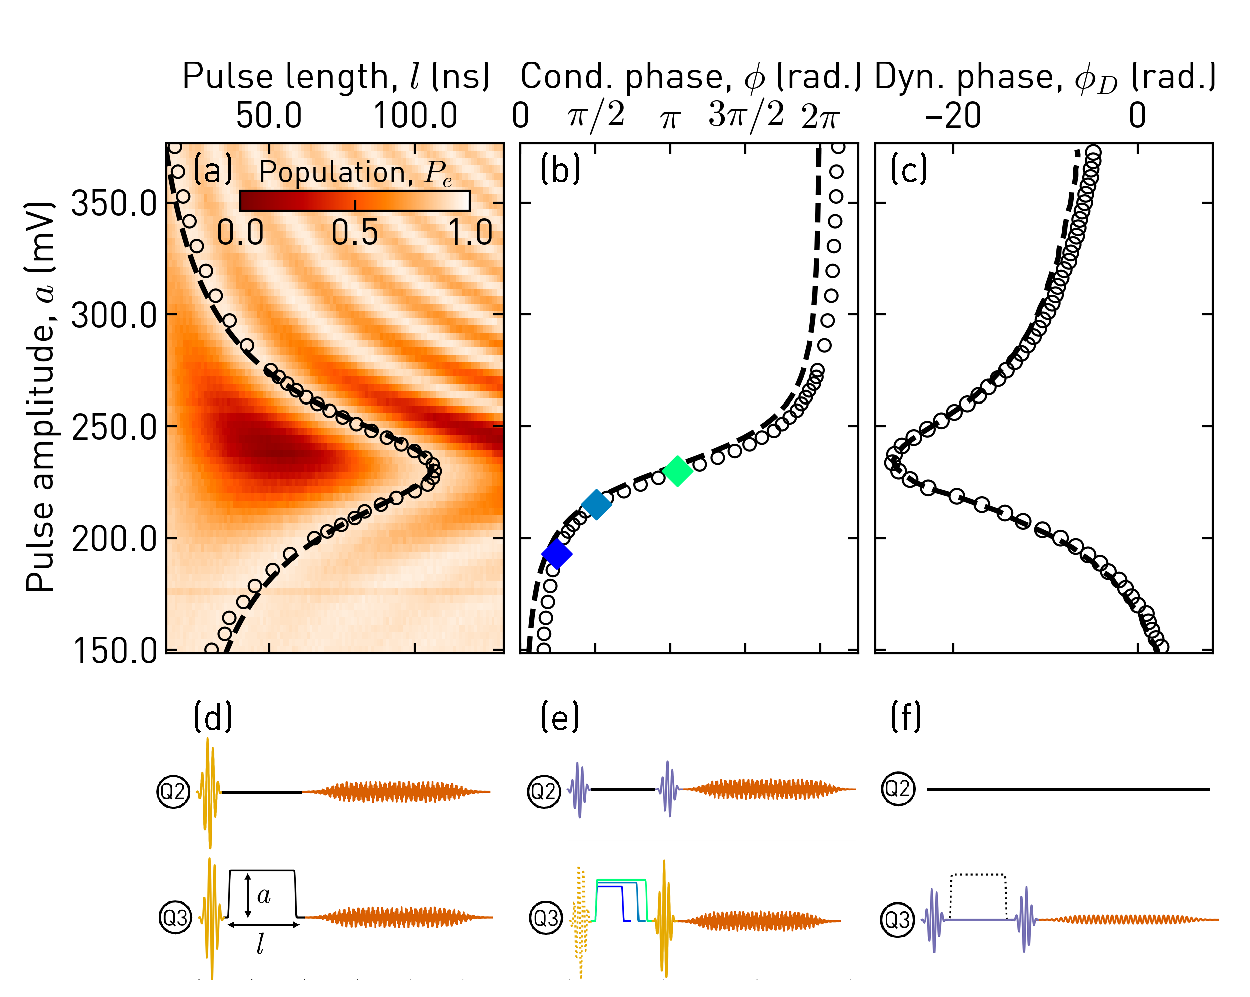
\includegraphics[width=\textwidth]{chapters/carb_gate/figs/ch4_carb_calibration_20200406_215519.pdf}
    \caption{Three calibration measurements (a, b, c) of a \gls{carb} and their corresponding pulse schemes (d, e, f).  (a) Qubit 2 \e{} level population as function of the flux pulse amplitude and length. The inset details the pulse scheme: the \oo{} state is prepared, the flux pluse (black) is  applied to qubit 3, the two qubits are read out with a multiplexed readout pulse. The scattered points correspond to the amplitudes and lengths used to calibrate the conditional phase (see b). The dashed line corresponds to the fit to the theoretical model. (b) Conditional phase as function of flux pulse amplitude. The amplitude sampling is not uniform to account for the non-linearity of the conditional phase. The dashed line indicates the phase predicted of the model (see main text for details).  (c) Unwrapped dynamic phase of qubit 3 as function of pulse amplitude. Only one out of three data point is shown for clarity.  The dashed line corresponds to the dynamic phase predicted by theory (see main text for details). (d) Pulse scheme corresponding to the two-dimensional parameter sweep shown in (a). The \oo{} state is prepared with two single-qubit $R_x^\pi$ (yellow), followed by the flux pulse (black) of amplitude $a$ and length $l$, and finally a readout pulse (orange). (e) Pulse scheme to measure conditional phase (see b). The phase is measured on qubit 2 with a Ramsey experiment (two $R_x^{\pi/2}$ pulses (purple)), while qubit 3 is fluxed once with and once without preceding single-qubit $R_x^{\pi}$ (dashed yellow). The difference between the two measurements yields the conditional phase. The different flux pulse colors result in the conditional phases indicated with diamonds of corresponding color in (b). (f) The dynamic phase is measured by comparing the phase of the qubit via a Ramsey experiment with and without flux pulse (dashed black).}
    \label{fig:ch4_calibration_carb}
\end{figure}

Due to flux cross-talk between the flux lines, the qubit staying at its parking position also acquires a non-zero dynamic phase. However, the latter is not calibrated, as flux cross-talk between the flux line of qubit 1 (3) and qubit 2 is smaller than 2\% (3\%) for the two two-qubit gates considered in this report~\cite{Andersen2018SampleB4QP3}.

The calibration time of the \gls{carb} on qubits 2 and 3 amounts to approximately 2 hours and 45 minutes i.e.\ about 5 to 8 times slower than a full calibration of a \gls{cz}. The high-resolution, two-dimensional amplitude/gate length sweep last for 1 hour, whilst for the conditional phase measurement (45 calibration points) requires 15 minutes, and the dynamic phase, 1 hour and 30 minutes. The following actions would reduce the calibration time:
\begin{itemize}
    \item[--] Use the active reset scheme discussed in Section~\ref{sec:active_reset}. This scheme allows an increase of the repetition rate by a factor of 5-10 leading to a total measurement time of 20-40 minutes.
    \item[--] Use a non-linear amplitude sampling for the dynamic phase based on the theoretical model. Namely, have an adaptable spacing between amplitudes at which the dynamic phase is calibrated based on whether the model predicts a large or small increase in dynamic phase. This would reduce the number of measurement point for the dynamic phase calibration by a factor of $\sim2$, compared to a dense linear pulse amplitude spacing.
    \item[--] Rewrite the dynamic phase measurement such that all waveforms are uploaded on the AWGs at once, instead of one at the time. This would reduce communication overhead.
\end{itemize}
Implementing these changes could in principle reduce the calibration time to under 20min per gate. Parallel tune up of two-qubit gates has the potential to decrease the calibration time of the device even further. 

In this section, we demonstrated the ability to calibrate a \gls{carb}. The next section details the characterization of the gate.

\begin{comment}
In addition to the pulse calibration, we use  \gls{iir} and \gls{fir} filters to predistort the pulses. compensate for the charge accumulation on the bias-tee and the frequency-dependent response of the flux line, we additionally pre-distort the pulse according to the procedure detailed in ~\cite{Butscher2018ShapingFiltering}
For the calibration of the \gls{iir} and \gls{fir} filters, which . The filters predistort the flux pulse to achieve the desired pulse shape at the quantum device.
\end{comment}

\section{Characterization} 
Randomized benchmarking -- the most common method to characterize two-qubit gates -- cannot be performed on the \gls{carb} because it is not part of the Clifford group~\cite{Magesan2011ScalableProcesses, Magesan2012CharacterizingBenchmarking}. Hence, we use another common method called quantum process tomography to characterize the \gls{carb}. Next, we perform a fine target phase sweep and characterize conditional and dynamic phase errors as well as leakage out of the computational subspace. Finally, we compare the performance of the \gls{carb} to the \gls{cz} and assess their  stability over a time (up to 15 hours after calibration).

\subsection{Quantum process tomography}
\Gls{qpt} is a method providing full description of a quantum process~\cite{Chuang1997PrescriptionBox, Poyatos1997CompleteGate}. In brief, it consists of preparing an ensemble of input states $\{\rho_1^\mathrm{in}, ..., \rho_k^\mathrm{in}\}$ spanning the Hilbert space of interest, passing them through the quantum process $\mathcal{E}$ and finally identifying the resultant states  $\{\rho_1^\mathrm{out}, ..., \rho_k^\mathrm{out}\}$ using quantum state tomography~\cite{Reed2013EntanglementQubits}. The output states are then
\begin{equation}
    \rho_k^{\mathrm{out}} = \mathcal{E}(\rho_k^\mathrm{in}) = \sum_{m n} \chi_{m n} P_n \rho_k^\mathrm{in} P_m^\dag
\end{equation}
 where $\chi$ is the process matrix and $P$ is the Pauli operator basis for 2 qubits: $P_n \in \{I, X, -\i Y, Z\}^{\otimes 2}$~\cite{HeinsooDigitalQubits}. The inversion of the above equation yields the desired process matrix $\chi$, which describes how the process affects an arbitrary input density matrix. 
 
The process fidelity $\mathcal{F}$ quantifies the closeness between the measured process matrix $\chi_\mathrm{exp}$ and the target matrix $\chi_\mathrm{targ}$~\cite{Schumacher1996SendingChannels}: 
 \begin{equation}
     \mathcal{F} = \mathrm{Tr}(\chi_\mathrm{exp} \chi_\mathrm{targ})
 \end{equation}
This metric quantifies how well the measured gate would act on half of a fully entangled system and if that action is identical to the target operation.
In the presence of leakage, the tomographic reconstruction of the computational subspace is not a trace-preserving map~\cite{Wood2018QuantificationErrors}. Therefore, we use the 3-level readout scheme discussed in Appendix~\ref{ch:qutrit_readout} to detect and exclude leakage events from the tomography measurement. We characterize leakage occuring during the gate separately in Section~\ref{sec:carb_characterization_phase_errors_leakage}. 
Readout noise can also lead to non-physical\footnote{A physical density matrix is positive semidefinite, Hermitian and trace preserving.} density matrix reconstructions. We use a maximum likelihood algorithm to find physical density matrices which are most likely to have been measured under the assumption of Gaussian noise~\cite{BaurRealizingQubits}. 
Finally, we correct for readout errors by multiplying the measured probabilities with the inverse of the readout probability matrix (see Section \ref{sec:qutrit_readout_correction} and Supplementary Material~\cite[suppl.~mat.]{Bialczak2010QuantumQubits}).

We perform \gls{qpt} for various target conditional phases of the \gls{carb}. Two resulting process matrices, $\chi^\pi$ and $\chi^{7\pi/4}$,  for target phases of $\pi$ and $7\pi/4$ respectively, are shown in Fig.~\ref{fig:carb_characterization_chi_matrices}. The black frame represents the target process matrices while the filled bars correspond to the reconstructed process matrices. We observe a good  agreement between them. In the chosen operator basis, a process matrix which can be described by a real unitary operator will also be real~\cite{Nielsen2000QuantumInformation}. This is the case for $\chi^\pi$, which is described by the real diagonal \gls{cz} unitary (see Eq.~\eqref{eq:carb_unitary} with $\phi = \pi$). By contrast, $\chi^{7\pi/4}$ is not described by a real unitary operator and therefore contains an imaginary part. On the diagonal of the real part, the same terms appear as in $\chi^{\pi}$, but with a different relative contribution. In particular, the $II$ contribution is higher, as adding a phase of $7\pi/4$ (nearly $2\pi$) on the \oo{} state is closer to an identity operation than adding a phase of $\pi$.

\begin{figure}[ht]
    \centering
    \includegraphics[width=\textwidth]{chapters/carb_gate/figs/process_tomography_chi_mtx.jpg}
    \caption{Real (a, c) and imaginary (b, d) elements of the process matrices $\chi^\pi$ and $\chi^{7\pi/4}$ respectively. The black wire frame corresponds to the target process matrix, while the blue (positive values) and red (negative values) filled bars correspond to the recontructed process matrix from measurements. The process fidelity for the phase  $\pi$ ($7\pi/4$) is 97.3\% (98.3\%).   }
    \label{fig:carb_characterization_chi_matrices}
\end{figure}

In Fig.~\ref{fig:carb_characterization_process_fidelity}, we show the process fidelity for 7 phase angles of the \gls{carb}. The maximum (minimum) fidelity is $98.3\%$ ($97.3\%$), for a phase of $7\pi/4$ ($\pi$). The expected fidelity from a master equation simulation including effects of decoherence during the gate is shown as dotted line. It explains about 1 \%, and is largest near phases of $\pi$. Thermal population  (0.4\% (1.3\%) at the time of the measurement on qubit 2 (3)) also affects the fidelity of the gate. Nevertheless, evaluating its effect precisely is not trivial: during \gls{qpt} the thermal population is mixed into other states with the tomography preparation pulses. Therefore, we scale the fidelity obtained by simulation by the probability that both qubits are in the ground state before starting the measurement. We suggest that this constitutes an approximate lower bound for the fidelity. This lower bound corresponds to the dashed line in Fig.~\ref{fig:carb_characterization_process_fidelity}. While this lower bound closely matches the measured fidelities near phases of $\pi$, it underestimates the fidelity for small and large phases. We expect this underestimation arises because both low and large conditional phase gates are closer to an identity operation and in the limit of a fully mixed (thermal) state, any gate behaves the identity operation. A detailed theoretical analysis is beyond the scope of this thesis (see e.g.~\cite{Korotkov2013ErrorTomography}).

\begin{figure}[ht]
    \centering
    \includegraphics[width=\textwidth]{chapters/carb_gate/figs/ch4_characterization_tomo_all_angles_20200406_144758.png}
    \caption{Process fidelity as function of conditional phase angle of the \gls{carb}. Measurements are shown in scattered points.  Master equation simulation including effects of decoherence in dotted line. The dashed line corresponds to the fidelity of the simulation scaled by the probability of starting the measurement in the ground state. }
    \label{fig:carb_characterization_process_fidelity}
\end{figure}

Although \gls{qpt} yields full information of the quantum process, it also has several downsides. It is a time-consuming measurement and does not provide a direct and intuitive explanation about the different origin of errors. In addition, the maximum likelihood estimation of the process matrix relies on the assumption that state preparation and measurement errors are negligible, which is not necessarily the case when the length of the two-qubit pulse is on the same scale as the single-qubit tomography pulses (i.e. for small and large target conditional phases). Finally, it does not include information about leakage. We therefore perform additional characterization measurements in the next section which portray leakage and phase errors directly.

\subsection{Phases errors and leakage} \label{sec:carb_characterization_phase_errors_leakage}
A natural way to test the gate before its usage in an algorithm is to target a conditional phase and assess how close the measured conditional phase is from the target. When using 3-level readout, this measurement also characterizes, for each target phase, the \f{} level population of the qubit leaving the computational subspace (in this case, qubit 2). A similar approach allows to assess how well we are able to predict the dynamic phase the fluxed-qubit acquires.

We perform such a sweep over a target conditional phase in the range $[0\degree, 360\degree[$ with a spacing of 8\degree{} and present the results in Fig.~\ref{fig:carb_characterization_phase_errors_leakage}(a). The conditional (dynamic) phase error shows a distribution with mean and standard deviation of $0.23\pm0.97\degree$ ($-0.28\pm1.38\degree$) respectively. To reduce the phase error even further, we could investigate different interpolation strategies. However, we argue that these phase errors will not be the limiting factor when used in algorithms. Indeed, the fidelity\footnote{We use the  definition of fidelity between two pure states $\psi_{\rho}$ and $\psi_{\sigma}$ as the squared overlap between the amplitudes: $\mathcal{F} = \left|\left\langle\psi_{\rho} | \psi_{\sigma}\right\rangle\right|^{2}$~\cite{Jozsa1994FidelityStates}. We define the gate fidelity as by the fidelity between the state resulting for the ideal gate and the state resulting from the faulty gate implementation, minimized over all input
states~\cite{Reiner2018EffectsSystems}.} of a gate subjected to an over-rotation $\delta\phi$ degrades with $\cos^2{\delta\phi}$~\cite{Reiner2018EffectsSystems}. Therefore, for $\delta\phi = 2 \degree \approx 2\sigma_{\textrm{err}}$, the expected infidelity is on the order of $0.1\%$ ($0.2\%$ when adding both conditional and dynamic phase errors). By comparison, the effect of decoherence leads to a 5 times larger infidelity, and the 400\unit{kHz} residual $ZZ$-coupling for a duration of $100 \unit{ns}$ induces a phase error of 14.4\degree{} on the \oo{} state\footnote{Note that errors resulting from residual $ZZ$-coupling do not accumulate during the two-qubit gate but rather during single-qubit pulses and idle time because the calibration of the conditional phase includes the phase resulting from residual $ZZ$-coupling}. 

The leakage population shows an angular dependency. It is minimal ($P_f \approx 10^{-3}$) for conditional phases far from 180\degree, namely when the gate is short and the \oo{} and \tz{} states are off-resonant. By contrast, we observe leakage of up to $2\%$ when the \oo{} and \tz{} states are near resonance. At resonance, the population transfer is maximal, leading to a maximum in leakage population when assuming a fixed probability excitations being trapped in the \tz{} state. The dominant source of leakage are the short timescale distortions of the flux pulse~\cite{Rol2019Time-domainProcessor} which are not perfectly compensated by the \gls{fir} filters used for pre-distortion~\cite{Butscher2018ShapingFiltering}.  Leakage of qubit 3, which does not go into the \f{} level during the pulse, is on the order of $10^{-4}$ for all target conditional phases.

\begin{figure}[ht]
    \centering
    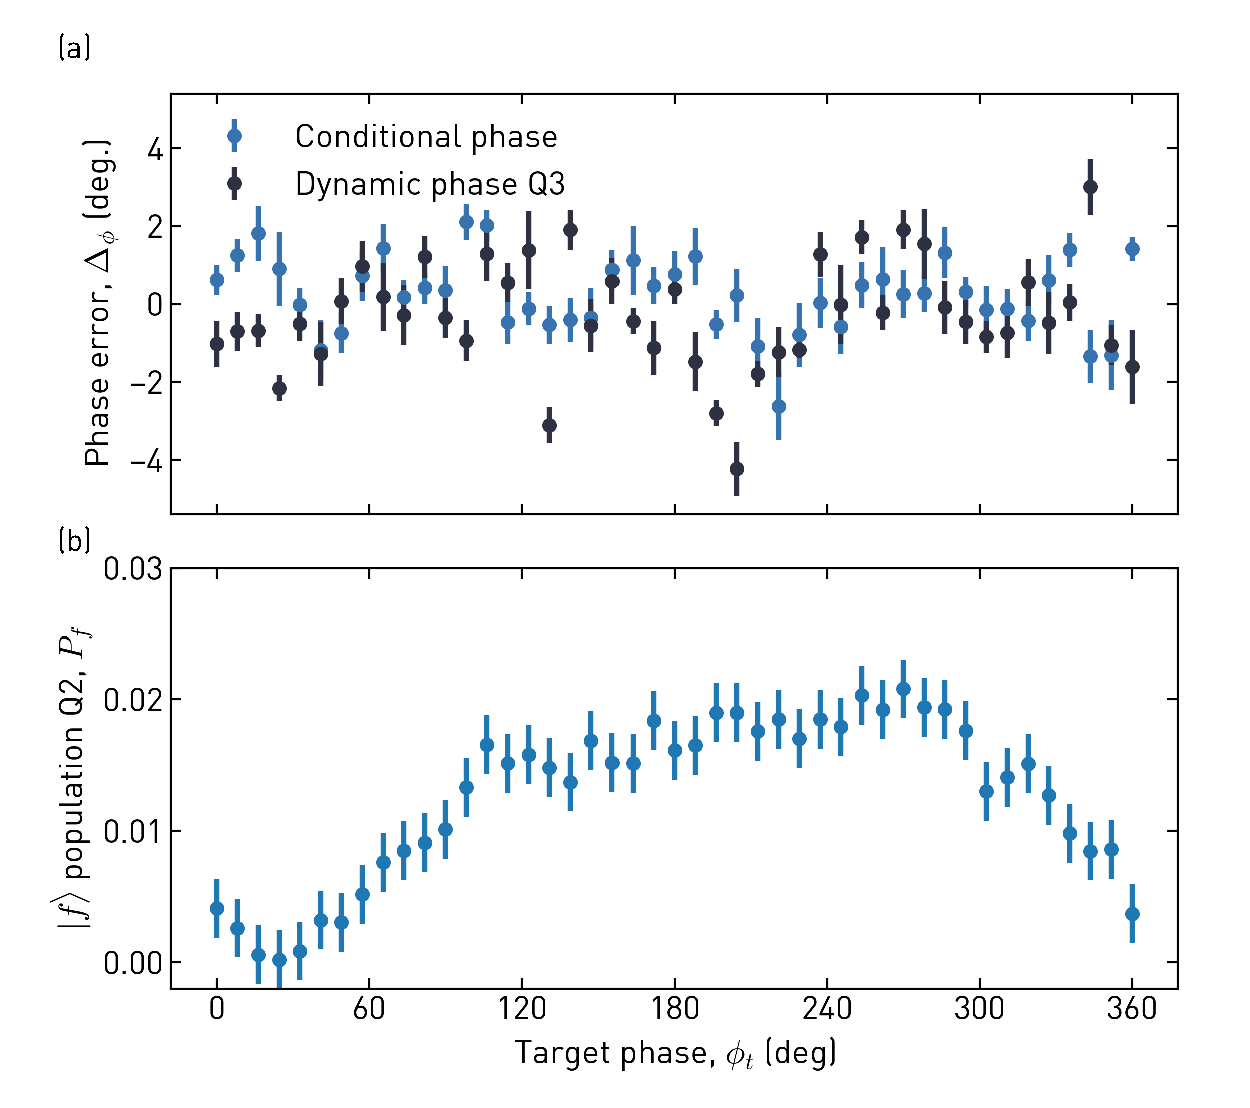
\includegraphics[width=\textwidth]{chapters/carb_gate/figs/ch4_characterization_phase_error_and_leakage_20200126_094856.pdf}
    \caption{Characterization of phase errors and leakage as function of target conditional phase with a granularity of 8\degree. Each point is averaged over 40000 single shots. (a) Conditional (light blue) and dynamic phase error (dark blue) show distributions with mean and standard distributions of $0.23\pm0.97\degree$ and  $-0.28\pm1.38\degree$ respectively. (b) We use 3-level readout to characterize leakage and measure up to 2\% leakage.}
    \label{fig:carb_characterization_phase_errors_leakage}
\end{figure}

\subsection{Comparison between C-ARB gates and CZ gates}
As final characterization procedure, we compare the \gls{carb} and \gls{cz} (implemented on the same qubits) in terms of phase errors, leakage and long term stability. We calibrate both gates and repeat the measurement described in Section~\ref{sec:carb_characterization_phase_errors_leakage}. For the \gls{cz}, we target a conditional phase of 180\degree, repeated $N$ times.  For the \gls{carb}, we sweep the range of target phases from 0 to 360\degree{} with $N$ points. These measurements are repeated for up to 15 hours after calibration. The full distributions of deviations from measured phases to target phases and leakages are presented as individual histograms, visualized as shaded filling in Fig.~\ref{fig:carb_characterization_drift}.

Both gates exhibit a similar range of conditional phase errors (standard deviation of $0.95\degree{}$ for the \gls{carb} versus $0.80\degree{}$ for the \gls{cz}). We conclude that extending the \gls{cz} to a \gls{carb} does not strongly impact the ability of preparing a target conditional phase. Note that the \gls{cz} shows a consistent offset of approximately 1\degree{} with respect to its target conditional phase. This originates from the fact that the gate is calibrated with a single point, which in this case was on the lower tail of the distribution. 

The \gls{carb} displays a wider distribution of dynamic phase errors, with an average standard deviation of 1.26\degree{} versus 0.83\degree{} for the \gls{cz}. This suggests it is harder to calibrate the dynamic phase for many flux pulse amplitudes and lengths simultaneously compared to calibrating only one. Preliminary analysis also suggest that the interpolation method has an influence on the standard deviation of the dynamic phase error. Using a cubic spline interpolation could help reduce the dynamic phase interpolation errors, compared to the implemented linear interpolation. 

The qubit 2 leakage trends are consistent with the discussion in Section~\ref{sec:carb_characterization_phase_errors_leakage}: the \gls{cz} experiences an average leakage of approximately 2\% since the \oo{} and \tz{} levels are on resonance. By contrast, the \gls{carb} experiences an average leakage of 1.4\% as several conditional phases result in low leakage. Its worse case leakage, however, is comparable to the one of the \gls{cz}. 

The phase error distributions stay relatively stable in time for both gates which suggests they will provide stable performance in algorithms for up to 15 hours after calibration.

The gates also differ in their average lengths. This effect is best visualized in Fig.~\ref{fig:ch4_calibration_carb}(a). While the \gls{cz} has a fixed flux pulse length of $107\unit{ns}$, the \gls{carb}'s flux pulse length is target phase dependent.  Averaged over all conditional phases, the flux pulse length is $84\unit{ns}$ long or $\sim 20\%$ shorter than for a conditional phase of 180 \degree. For both implementations, we add a $10\unit{ns}$ ($15\unit{ns}$) buffer at the start (end) to avoid overlap of other gates with the rising and falling edges of the flux pulse.

\begin{figure}[ht]
    \centering
    \includegraphics[width=\textwidth]{chapters/carb_gate/figs/ch4_characterization_drift_20200124_175455.png}
    \caption{Comparison between the \gls{cz} (green) and \gls{carb} (blue) in terms of phase errors and leakage as a function of time elapsed since calibration. The error bars correspond to the mean and standard deviation while the full distribution ($N$ = 45 points) is shown as shaded filling.}
    \label{fig:carb_characterization_drift}
\end{figure}

\section{Conclusion}
 In this chapter we have shown how to achieve a two-qubit unitary operation $U_{\textrm{C-ARB}}$ which adds an arbitrary phase $\phi$ on the \oo{} state. We implement this unitary by varying the frequency detuning between the \oo{} and the non-computational \tz{} state with a square,  Gaussian-filtered flux pulse. We adjust the length of the flux pulse to ensure high population recovery in the computational subspace. In practice, we calibrate the gate for a finite number of conditional phases (45) and interpolate linearly all parameters to reach phases between the calibration points. 
 
 We have characterized the gate using quantum process tomography for different conditional phases yielding a fidelity between 97.3\% and 98.3\%. The infidelity is dominated by decoherence and thermal population. In addition, we have shown that phase errors are small compared to other error mechanisms such as decoherence and residual $ZZ$-coupling. The average leakage amounts to 1.4\% and originates from the distortions of the flux pulse which are not corrected by the finite impulse response filter. The \gls{carb} shows similar time stability and phase error distributions as a \gls{cz} implemented on the same qubits while being 20\% shorter on average. 
 
 Although its calibration procedure is more elaborate, the \gls{carb} enables a significant gate count reduction for of \gls{vqa} circuits. In the next chapter, we implement a three-qubit problem instance which we solve using the \gls{qaoa} to demonstrate this advantage.



\chapter{Solving an exact cover problem using the QAOA} \label{ch:qaoa}
An optimization problem where the aim is to find the optimal (or close to optimal) solution amongst a finite set of possibilities is called a \textit{combinatorial optimization problem}.  Such problems are pervasive and appear in applications such as green logistics, hardware verification, task scheduling and telecommunication network design \cite{Sbihi2007CombinatorialA, Coles2018QuantumBeginners, 2014ApplicationsOptimization}.

In this chapter, we first introduce the notion of combinatorial optimization. Next, we explain the \gls{qaoa}, a quantum heuristic algorithm providing approximate solutions to combinatorial optimization problems. We show that using \glspl{carb} can reduce the length of \gls{qaoa}'s gate sequence implemented on the quantum computer. This allows for more complex algorithms to be run on the quantum computer compared to when only \gls{cz} are used. Next, we demonstrate this advantage experimentally by solving a combinatorial optimization problem called exact cover on a three qubit quantum processor.

\section{Combinatorial optimization}
It its general form, a combinatorial optimization problem is specified by a set of rules, called clauses, acting on strings of $N$ bits, in which each bit represents a binary decision variable \cite{Farhi2014AAlgorithm}.  Each clause is satisfied for certain assignments of the bits and unsatisfied for other assignments. Solving the problem consists in finding a combination of bits (forming together the bit string) satisfying the largest (weighted) amount of clauses. The objective function can be written as 
\begin{equation}
    C(b) = \sum_{m=1}^M w_m C_m(b)
\end{equation}
where $b = b_1 \, ...\, b_N$ the bit string,  $C_m(b)$ is the $m$-th clause and $w_m$ is its corresponding (real and non negative) weight. If $C_m(b)$ is satisfied by the bit string $z$ then its value is 1 and otherwise 0. In these terms, solving the problem is expressed as finding the bit string $b_\text{opt}$ maximizing C. An approximate solution provides a bit string $b_{\text{approx}}$ for which  $C(b_{\text{approx}})$ is close to the maximum of C.

We illustrate this abstract concept with a simple example. Imagine you are going to a party, and have to choose an outfit -- consisting of one t-shirt and one pair of pants -- from your closet. You have 2 shirts to choose from, a black (0) and white (1) one. Similarily, you have a black (0) and a white (1) pair of pants. You believes you look better when your whole outfit is of the same color. Additionally, you  believe your white shirt suits you better than the black one. Which outfit should you choose for the party? 

While the answer is trivial in this example, we formalize the problem with the terminology introduced above. The outfit, $b$, can be formulated as a 2-bit string, one bit for the shirt ($b_1$), and one for the pair of pants ($b_2$). Colors are encoded by the values of the bits: 0 for black and 1 for white. The four possible outfits are: 00 (black-black), 01 (black-white), 10 (white-black) and 11 (white-white). The problem has two clauses. $C_1(b) := b_1 \oplus b_2$, leading to a value of 1 if you choose a shirt and pair of pants of the same color and 0 otherwise\footnote{$\oplus$ denotes the "XOR" operation, which gives an output of 1 if and only if the two inputs are 11 or 00}. $C_2(b) := b_1$ has a value of 1 if you chooses your white shirt. The objective function is then:
\begin{equation}
    C(b) = C_1(b) + C_2(b) = (b_1 \oplus b_2) + b_1
\end{equation}
where we assigned equal weights $w_1 = w_2 = 1$ to both clauses.
The score of each output is then:
\begin{subequations}
\begin{equation}
     C(00) = 1 + 0 = 1
\end{equation}
\begin{equation}
    C(01) = 0 + 0 = 0
\end{equation}
   \begin{equation}
       C(10) = 0 +  1 = 1
   \end{equation}
   \begin{equation}
         C(11) = 1 + 1 = 2
   \end{equation}
\end{subequations}

The bit string maximizing $C(b)$ is indeed 11 (white shirt, white pants). An algorithm capable of providing this bit string is a combinatorial optimization algorithm. In this case, we used the \textit{exhaustive search} algorithm, meaning that we enumerated all possible answers and picked the best one. 

In many real applications, exhaustive search is not tractable. In fact, even a slight modification of the presented problem makes it unrealistic to use exhaustive search. Imagine having to choose 25 items, each possible in 8 different colors (each item has now 3 bits to encode the colors). The number of possible outfit is the $2^{3 \cdot 25} \simeq 4\cdot 10^{22}$! It would take about a million years to search through all possibilities for a computer requiring $1\unit{ns}$ per outfit.

There exist several (classical) heuristic algorithms providing an approximate solution for this type of problems. In the next section, we explain the \gls{qaoa}, a quantum heuristic algorithm capable of finding approximate solutions to this type of problems.

\section{The quantum approximate optimization algorithm}\label{sec:qaoa}
The \gls{qaoa} \cite{Farhi2014AAlgorithm} (depicted in Fig. \ref{fig:qaoa_scheme}a) is a \gls{vqa} designed to find approximate solutions to combinatorial optimization problems. It is a hybdrid algorithm executed partially on a quantum and partially on a classical computer. 

First, the quantum computer prepares a quantum state $\ket{\vec{\gamma}, \vec{\beta}}$ based on the objective function\footnote{Also sometimes named cost function} $C$ characterizing the problem and a set of variational parameters $\theta = (\vec \gamma, \vec \beta)$. The state is prepared with $p$ layers of two non commuting Hamiltonians, $\hat C$ and $\hat B$, applied to a uniform superposition state of $N$ qubits:
\begin{equation}
    |\vec{\gamma}, \vec{\beta}\rangle=\underbrace{e^{-i \beta_{p} \hat B} e^{-i \gamma_{p} \hat C}}_{\text {layer } p} \cdots \underbrace{e^{-i \beta_{1} \hat B} e^{-i \gamma_{1} \hat C}}_{\text {layer } 1}|+\rangle^{\otimes N}
\end{equation}
where $\vec\gamma = (\gamma_1, ..., \gamma_p)^\text{T}$ and $\vec\beta = (\beta_1, ... , \beta_p)^\text{T}$ are the real variational parameters for the $p$ layers. Referring to the number of layers, we say that the implementation is of depth $p$. $\hat C$ is the cost Hamiltonian, which for all objective functions of NP-complete problems can be mapped in polynomial time to an Ising Hamiltonian \cite{Lucas2014IsingProblems},
\begin{equation}
    \hat C =\sum_{n < m} J_{n m} \sigma_{n}^z \sigma_{m}^z + \sum_{n} h_n \sigma_{n}^z
\end{equation}
and $\hat B$ is the mixing Hamiltonian 
\begin{equation}
    \hat B = \sum_{n} \sigma_n^x
\end{equation}
where $\sigma_n^{z (x)}$ are the Pauli Z (X) operators applied to the $n$-th qubit, and $h_n$ and $J_{n m}$ are real coefficients.

The resulting state \qaoaMeasuredState{} is then measured in the $Z$ basis. A classical computer uses the measurement outcome to compute the expectation value of $\hat C$ and iteratively updates the variational angles to optimize the objective function. When the objective function is mapped to the Ising Hamiltonian, the resulting problem consists in finding the lowest energy state of the system, i.e. minimizing the expectation value of the cost Hamiltonian. Once the algorithm has converged, the state \optimalstate{} is an approximate solution for the objective function $C$.

\begin{figure}
    \centering
    \includegraphics[width=\textwidth]{chapters/qaoa/figs/qaoa_scheme.png}
    \caption{The \gls{qaoa} scheme. (a) The scheme consists of two steps. First, the quantum computer applies $p$ alternating sequences -- called layers -- of two Hamiltonians ($\hat C$ and $\hat B$) scaled by layer-dependent variational parameters to an equal superposition state. The resulting state, $\ket{\vec\gamma,\vec\beta}$, is prepared and measured several time to obtain an estimate for the expectation value of a cost function \cost, based on the expectation values of single and two qubit terms. Based on this estimate, a classical optimizer alters the variational parameters to minimize \cost. The output of the algorithm is the projection of state \optimalstate yielding an bit-string which cost is small. }
    \label{fig:qaoa_scheme}
\end{figure}
\subsection{The importance of depth}
The depth of a \gls{qaoa} implementation is defined as the number of layers, $p$, used for the state preparatation.

For $p \rightarrow \infty$, the \gls{qaoa} finds the global optimium of $C$ \cite{Farhi2014AAlgorithm}. Intuitively, this is because the \gls{qaoa} can be seen as a Trotterized approximation \cite{TrotterMathematics} of the quantum adiabatic algorithm \cite{Farhi2000QuantumEvolution}. Similarly to the \gls{qaoa}, the quantum adiabatic algorithm starts in the highest energy state of the mixing Hamiltonian $\hat B$, i.e. equal superposition over all qubits in the $Z$ basis, and then evolves adiabatically to the cost Hamiltonian $\hat C$,
\begin{equation} \label{eq:qaoa_adiabatic_evolution}
\sexp{-\i \hat H(t)\,t}= \sexp{-\i \left(\hat H_1(t) +\, \hat H_2(t)\right) \, t} = \sexp{-\i \left((1-t / T) \hat B+ \, (t / T) \hat C\right)\, t}
\end{equation}
where $T$ is a real and positive parameter called run time. As long as the evolution is sufficiently slow i.e. $T$ is sufficiently large, this process forces the state of the system to remain in the ground state of the slowly varying Hamiltonian $\hat H(t)$, ultimately resulting to the ground state of $\hat C$ \cite{Farhi2000QuantumEvolution, Farhi2014AAlgorithm}. \gls{qaoa} is a trotterized approximation of this evolution, where the Trotter product formula stipulates that for two \textit{time independent} Hamiltonians $\hat H_1$ and $\hat H_2$ \cite{TrotterMathematics}:
\begin{equation} \label{eq:qaoa_product_formula}
    \sexp{-\i\left(\hat H_{1} + \hat H_{2}\right) t}=\lim _{K \rightarrow \infty}\left(\sexp{-\i \hat H_{1} t / K} \sexp{-\i \hat H_{2} t / K}\right)^{K}
\end{equation}
Truncating this equation to a finite value for  $K$ yields an error $\epsilon$ with lowest order term in $\mathcal{O}\left(\frac{t^2}{2K} [\hat H_1, \hat H_2]\right)$ \cite{Heyl2018QuantumSimulation, Lloyd1996UniversalSimulators}.

To relate this forumla to the time evolution of Eq. \eqref{eq:qaoa_adiabatic_evolution}, we approximate $\hat H_1(t)$ and $\hat H_2(t)$ by piecewise constant Hamiltionians that take the value $\hat H_i(l\Delta \tau)$ for $i = 1,2$ over intervals of length $\Delta \tau$ such that
\begin{equation} \label{eq:qaoa_discretization}
    \sexp{-\i\left(\hat H_{1}(t) + \hat H_{2}(t)\right) t} \approx \prod_{l = 1}^L \sexp{-\i\left(\hat H_{1}(l\,\Delta \tau) + \hat H_{2}(l\,\Delta \tau)\right) t}
\end{equation}
This approximation is valid as long as $\Delta \tau \ll\|\partial \hat H(t) / \partial t\|^{-1}$ \cite{Poulin2011QuantumSpace}, namely as long as time fluctuations in $H$ are small on the interval $\Delta \tau$.

Then, we use Eq. \eqref{eq:qaoa_product_formula} with $K = 1$ to decompose each matrix exponential,
\begin{equation}
    \sexp{-\i\left(\hat H_{1}(l\,\Delta \tau) + \hat H_{2}(l\,\Delta \tau)\right) t} = \sexp{-\i\hat H_{1}(l\,\Delta \tau)t}\cdot \sexp{\hat H_{2}(l\,\Delta \tau) t} + \epsilon 
\end{equation}
Combinating this first order trotter approximation with  Eq. \eqref{eq:qaoa_discretization} and Eq. \eqref{eq:qaoa_adiabatic_evolution} yields for the full time evolution:
\begin{equation}
    \prod_{l=1}^L\sexp{-\i\overbrace{(1-l\Delta\tau/T)\Delta\tau}^{\gamma_l}\hat C} \cdot \sexp{-\i\overbrace{(l\Delta\tau/T)\Delta\tau}^{\beta_l}\hat B} 
\end{equation}

PROBLEM: C and B are in reversed order. so last equation does not work, also should define $U(t1, t2) $ to indicate evolution from t1 to t2. 

have more layers = longer run time T for fixed delta t (or shorter delta t for same run time?)
-relate christian depth grows in logN, + chuang investigation of depth.

\subsection{Speedup}
At the time of its publication, the \gls{qaoa} achieved a higher approximation ratio on MAX-3-LIN-2 -- a specific instance of the NP-complete MaxCut problem \cite{GareyM1990} -- than any other classical algorithm. This is no longer the case \cite{Barak2015BeatingDegree, Hastings2019CLASSICALALGORITHMS}. In fact, several work have shown that classical algorithms could outperform the \gls{qaoa} on a variety of problem instances \cite{Barak2015BeatingDegree, Hastings2019CLASSICALALGORITHMS, Bravyi2019ObstaclesProtection}. On the other hand, several work claim to achieve Grover speedup for unstructured search \cite{Jiang2017Near-optimalField} and state transfer \cite{Niu2019OptimizingDepth}. Whether or not the \gls{qaoa} will provide a provable or practical speedup compared to classical algorithms remains an open research question.

Nevertheless, the \gls{qaoa} remains one of the most studied \gls{vqa} in literature -- both theoretically and experimentally. It is therefore a good candidate to illustrate the advantage of \glspl{carb} and compare their performance with other published experiments. 


- introduced by Farhi, extension to ansatz
- scaling, why we want it
- idea of two non commuting hamiltonians
- trotterization : https://vtomole.com/blog/2019/04/07/trotter 
- explain flow
- role of p
- work on influence of p for large problems
- christian scaling of p with number of qubits

\subsection{Success probability}
Measuring successive preparations of \optimalstate yields a distribution of projected states $\ket{\psi_i}$.
We define the success probability, $P_s$, as the probability of measuring a projected state that is a solution to the combinatorial problem. 

Note that the optimization is performed on the smooth landscape of \cost{} and not on $P_s$ directly. But for problems with discrete domain of real values, a low expectation value of the cost function generally guarantees a high concentration of probability on optimal solutions upon measurement \cite{Cook2019TheCover, Wang2019XY-mixers:QAOA}.

\subsection{Cost hamiltonian with CZ/CARB}



\section{Experiment}
In this section, we implement the \gls{qaoa} on a quantum processor to find an approximate solution to a combinatorial optimization problem with 3 qubits. We use qubits 1, 2 and 3 of the device presended in Appendix \ref{app:device}. Information relative to the single- and two-qubit gates are reported in Appendix \ref{app:gate_parameters}. All measurements are performed with 3-level single shot readout. In the context of the \gls{qaoa}, leakage events can be seen as measuring bit strings which do not belong to the space of possible solutions. We therefore discard measurements in which one or several of the qubits are measured in the $f$-level. Hence leakage events reduce the effective number of shots on which we compute estimates. They do not, however, influence the algorithm as long as as the excitation stays in the f-level until the state is measured. We make this assumption, as sequences of interest are shorter than 4 micro-seconds, and the shortest f-level \t1 is approximately 10 micro-seconds. All measurements are done without ground state heralding or readout error correction.

After introducing the combinatorial problem, we assess how the direct and decomposed implementations of the arbitrary phase gate affect the performance of the algorithm for different depths. We show that the direct implementation allows to solve the problem more effectively than the decomposed implementation, because more layers can be implemented for a fixed algorithm sequence length. 

\subsection{Exact cover: definition and example problem instance}
We use \gls{qaoa} to find an approximate solution to an instance of the exact cover problem. The exact cover \cite{Karp1972ReducibilityProblems} is an NP-complete \cite{GareyM1990} decision problem formulated as follow: \textit{given a set $\mathcal{N}$, and a collection $\mathcal{L}$ of subsets of $\mathcal{N}$, is there a subcollection $\mathcal{L}'$ of $\mathcal{L}$ for which each element in $\mathcal{N}$ is included exactly once?} In other words, elements of the subcollection $\mathcal{L}'$ must be disjoint and their union must be $\mathcal{N}$.

As mentioned in Section \ref{sec:qaoa}, any NP-complete can be mapped onto an Ising Hamiltonian in polynomial time. For the exact cover, it is most conviently done using an incidence matrix $M$ \cite{WeissteinIncidenceMatrix}, where each row corresponds to an element of $\mathcal{L}$ and each column to an element of $\mathcal{N}$. The matrix element $M_{ln}$ is equal to 1 if the $l$-th element of $\mathcal{L}$ contains the $n$-th element of $\mathcal{N}$ and 0 otherwise.
The Ising parameters $J_{nl}$ and $h_l$ are obtained from $M$ \cite{Lucas2014IsingProblems, Vikstal2019ApplyingProblem}:
\begin{subequations}
\begin{equation}
    J_{l n}=\frac{1}{2} \sum_{k=1}^{N} M_{l k} M_{n k}
\end{equation}
\begin{equation}
h_{l}=\frac{1}{2} \sum_{n=1}^{N} M_{l n}\left(\sum_{k=1}^{L} M_{k n}-2\right)
\end{equation}
\end{subequations}
This formulation results in $L = |\mathcal{L}|$ spins in the Ising Hamiltionian, and each spin is mapped to a qubit. 

In this work, we consider the 3-qubit problem instance depicted in Fig. \ref{fig:qaoa_exact_cover_matrix}.  $\mathcal{N} := \{1,2,3\}$ and the elements of $\mathcal{L}$ are $A := \{1,2\},\,\, B := \{1,2,3\}$ and $C := \{2,3\}$, encoded in qubit 1, 2 and 3 respectively. In this picture, the decision problem becomes: \textit{is there a subcollection $\mathcal{L}'$ of letters for which each number in $\mathcal{N}$ is included exactly once?} The answer is yes, and the corresponding subcollections are $\mathcal{L}_1' = \{B\}$ and $\mathcal{L}_2' = \{A,C\}$. These subcollections are encoded in the states $\ket{\psi}=\ket{010}$ and $\ket{101}$, where a 1 in position $l$ indicates that the $l$-th element of $\mathcal{L}$ is included in the subcollection $\mathcal{L'}$.

\begin{figure}[ht]
    \centering
    \includegraphics[width=\textwidth, trim={11cm 8cm 38cm 10cm},clip]{chapters/qaoa/figs/exact_cover_matrix.pdf}
    \caption{Incidence matrix representation of the exact cover problem instance implemented in this work. A dot in indicates a 1 and an empty square indicates a 0. The mapping to the 3 qubit chain and the corresponding Ising Hamiltonian parameters are indicated on the right handside.}
    \label{fig:qaoa_exact_cover_matrix}
\end{figure}

The resulting cost Hamiltonian is
\begin{equation}
    \hat C = \frac{1}{2}\hat\sigma_1^z\hat\sigma_2^z + \hat\sigma_2^z\hat\sigma_3^z
\end{equation}
and the corresponding cost function $\cost = \bra{\vec\gamma, \vec\beta} \hat C \qaoaMeasuredState{}$ reaches its minimum value of $-1.5$ when $\qaoaMeasuredState{} = \ket{101}$ or $\ket{010}$. 

From noise-free simulations of the unitary evolution combined with brute force optimization, we observe that the problem requires 3 layers to achieve a success probability larger than 99\%.

In the following sections, we present the results of the i
explain experiment and goal to compare both implementations
-refer to appendix for details about device and two qubit gates params
- describe that we remove leakage.


\section{Optimization landscapes ($p$ = 1)}
In Fig. \ref{fig:qaoa_landscapes}, we present the optimization landscapes for a \gls{qaoa} implementation with one layer. 
\begin{figure}[ht]
    \centering
    \includegraphics[width=\textwidth]{chapters/qaoa/figs/qaoa_landscapes_20200129_125251.png}
    \caption{Landscapes}
    \label{fig:qaoa_landscapes}
\end{figure}
- landscapes
- simulation
- local minimas
- intuition for parameters space shape

\section{Init from random}
\begin{figure}[ht]
    \centering
    \includegraphics[width=\textwidth]{chapters/qaoa/figs/ch5_qaoa_optimization_traces_20200116_165916.png}
    \caption{Optimization landscapes for a \gls{qaoa} implementation with one layer. The two variational parameters, $\gamma$ and $\beta$ are swept with a 45x45 grid. Each pixel consists of the expectation value of the cost function obtained from 20000 single shots. (a) Landscape obtained with noise-free simulation. Clear local minima appear for values of $\gamma$ larger than $\pi/4$. The minimal cost function value is approximately -1.05. (b) Landscape obtained with the direct implementation. }
    \label{fig:qaoa_optimization_traces}
\end{figure}
- discuss optimizer, say what other used, what is important (low sampling, noise robust, avoid local minima)
- compare as function of p energy for both implementations

\section{Success prob as function of depth}


\begin{figure}[ht]
    \centering
    \includegraphics[width=\textwidth]{chapters/qaoa/figs/ch5_qaoa_sequence_lengths_v1_withinset_20200202_120000.png}
    \caption{Success probability as function of sequence length}
    \label{fig:qaoa_sequence_lengths}
\end{figure}

\begin{figure}[ht]
    \centering
    \includegraphics[width=\textwidth]{chapters/qaoa/figs/ch5_qaoa_state_histograms_20200202_134816.pdf}
    \caption{Landscapes}
    \label{fig:qaoa_state_histogram}
\end{figure}
\section{Conclusion}

\chapter{Conclusion}
\glsresetall{}

% Large-scale, fault-tolerant quantum computing has the potential to impact numerous fields such as chemistry, medical research, material science, information security and logistics. However, building large-scale and noise-free quantum computers is a substantial challenge. Consequently, near-term quantum computers will only have a limited number of quantum bits (qubits) and a limited computing time during which operations are executed reliably.

% \Glspl{vqa} are good candidates to take advantage of the quantum hardware in the near-term because they offset part of the computation to classical computers and are intrinsically more robust to noise mostly because they seek approximate solutions. The available computation time remains nevertheless limited by time-dependent errors such as decoherence and residual $ZZ$-coupling.

In  this  thesis,  we  demonstrated  a  way  to  enhance  the  performance  of \glspl{vqa} by reducing the  sequence length  required  to implement their circuit on quantum hardware. In particular, we enlarged the gate-set available on the quantum computer with a \gls{carb}, which enables us to avoid decomposition of higher order operations into multiple gates. 

The \gls{carb} is a generalized version of the controlled $\pi$-phase two-qubit gate (CZ gate). It is able to reach any phase on the \oo{} state between 0 and $2\pi$. Our implementation achieves an average process fidelity of 97.7\%, whereby the remaining errors are dominated by decoherence and effects of thermal population. The average leakage per gate amounts to 1.4\%, which is slightly lower than the leakage we obtain for a CZ gate implemented on the same physical qubits.

We demonstrated the advantage of \gls{carb} on a three qubit exact cover problem instance which we solved using the \gls{qaoa}, a \gls{vqa} that finds approximate solutions to combinatorial problems.  The instance we considered is the first experimental implementation requiring three QAOA layers to be solved with high success probability. 

We obtain a 50\% two-qubit gate count reduction and a gate sequence length reduction factor of 3 using the direct implementation of the \gls{carb} compared to a decomposition into \glspl{cz} and single qubit gates. Consequently, we achieve a higher success probability with the direct implementation (0.84 versus 0.64) because it executes more layers for a fixed sequence length. 

We foresee an even more pronounced advantage for larger-scale experiments because the number of layers required to solve problems typically scales with the number of qubits involved in the experiment. Therefore, for as long as quantum devices are limited by decoherence, \glspl{carb} will open the door to solving more complex problem instances with \gls{vqa}.

\appendix

\chapter{Setup}
\label{app:setup}

\begin{figure}[htp]
  \centering
 \includegraphics[width=0.8\textwidth]{appendices/figs/BF1_device.png}
 \caption{An optical micrograph of the 4-qubit device. Adapted from \cite{Andersen2019a}}
 \label{fig:BF1_device_picture}
\end{figure}

\begin{table}[ht]
\centering
\caption{Coherence, frequency, coupling, and readout properties of the device. The $T_1$ and $T_2$ times are measured at the maximum qubit frequency for qubit 1, and at the minimum qubit frequency for qubits 3 and 4. Qubit 2 is not tunable. Adapted from \cite{Andersen2019a}}
\begin{tabularx}{\textwidth}{llllll}
\toprule
Parameter & Unit & \textbf{Q1} & \textbf{Q2} & \textbf{Q3} & \textbf{Q4} \\ 
\midrule
Maximum qubit frequency & (GHz) & \multicolumn{1}{c}{5.721} & \multicolumn{1}{c}{5.210} & \multicolumn{1}{c}{5.530} & \multicolumn{1}{c}{5.160} \\
Minimum qubit frequency & (GHz) & 5.083 & 4.880 & 4.386 &  \\
Qubit lifetime & ($\mu$s) & 25.11 & 10.3 & 23.6 & 43.1 \\
Qubit Ramsey coherence time & ($\mu$s) & 23.87 & 11.3 & 14.2 & 10.7 \\
Qubit echo coherence time & ($\mu$s) & 34.8 & 12.1 & 19.5 & 20.2 \\
Readout resonator frequency & (GHz) & 6.892 & 7.087 & 6.687 & 6.487 \\
Purcell resonator – readout resonator detuning & (MHz) & 29.5 & 27.5 & 19.4 & 7.8 \\
Purcell resonator – readout resonator coupling & (MHz) & 10.9 & 8.2 & 9.5 & 10.4 \\
Purcell resonator to half-feedline coupling & (MHz) & 27.2 & 34.7 & 10.7 & 19.8 \\
Effective readout resonator linewidth & (MHz) & 2.4 & 2.0 & 1.5 & 6.1 \\
Dispersive shift & (MHz) & -3.9 & -1.6 & -1.8 & -2.4 \\
Thermal population & (\%) & 0.9 & 1.4 & 1.4 & 7.4 \\ 
\bottomrule
\end{tabularx}
\end{table}


\backmatter

\bibliographystyle{plain}
\bibliography{ressources/references_mendeley}

\includepdf[pages={-}]{declaration-originality.pdf}

\end{document}
